% Canonical manuscript source: two-column IEEEtran layout with the abstract in
% the first column and IEEE author blocks.
% Build from this folder with three passes of pdflatex; the generated PDF is
% fqcnn.pdf. Figures are read from the repository-level figs_final/ folder.
\documentclass[conference]{IEEEtran}
\IEEEoverridecommandlockouts
\usepackage{cite}
\usepackage{amsmath,amssymb,amsfonts}
\usepackage{amsthm}
\newtheorem{theorem}{Theorem}
\newtheorem{proposition}{Proposition}
\usepackage{algorithmic}
\usepackage{graphicx}
\graphicspath{{../}}
\usepackage{textcomp}
\usepackage{xcolor}
\usepackage{booktabs}
\usepackage{bm}
\usepackage{algorithm}
\definecolor{ieeelink}{RGB}{0,68,153}
\usepackage[colorlinks=true,allcolors=ieeelink,breaklinks=true]{hyperref}
% Make each reference number [n] in the bibliography an external link to the
% article DOI. In-text \cite numbers remain internal links to the entry.
\makeatletter
\@namedef{fqcnndoi@1}{https://doi.org/10.1103/PRXQuantum.3.010313}
\@namedef{fqcnndoi@2}{https://doi.org/10.1038/s41534-022-00592-6}
\@namedef{fqcnndoi@3}{https://doi.org/10.1038/s41534-025-00960-y}
\@namedef{fqcnndoi@4}{https://doi.org/10.1103/PhysRevLett.128.080506}
\@namedef{fqcnndoi@5}{https://doi.org/10.1103/PhysRevResearch.6.033029}
\@namedef{fqcnndoi@6}{https://doi.org/10.1103/RevModPhys.95.045005}
\@namedef{fqcnndoi@7}{https://doi.org/10.1038/s41534-024-00865-2}
\@namedef{fqcnndoi@8}{https://doi.org/10.1088/2058-9565/aa8072}
\@namedef{fqcnndoi@9}{https://doi.org/10.1016/j.automatica.2022.110659}
\@namedef{fqcnndoi@10}{https://doi.org/10.1038/s41567-019-0648-8}
\@namedef{fqcnndoi@11}{https://doi.org/10.1038/s41467-018-07090-4}
\@namedef{fqcnndoi@12}{https://doi.org/10.1038/s42254-021-00348-9}
\@namedef{fqcnndoi@13}{https://doi.org/10.1038/s41534-018-0116-9}
\@namedef{fqcnndoi@14}{https://doi.org/10.1038/s41467-021-21728-w}
\@namedef{fqcnndoi@15}{https://doi.org/10.1109/5.726791}
\renewcommand{\@biblabel}[1]{%
  \begingroup\edef\fqcnn@u{\csname fqcnndoi@#1\endcsname}%
  \expandafter\href\expandafter{\fqcnn@u}{[#1]}\endgroup}
\makeatother
\def\BibTeX{{\rm B\kern-.05em{\sc i\kern-.025em b}\kern-.08em
    T\kern-.1667em\lower.7ex\hbox{E}\kern-.125emX}}
\begin{document}

\title{FQCNN: A Fully Quantum-Native Convolutional Neural Network with Coherent Unitary Pooling}

\author{\IEEEauthorblockN{Aasa Singh Bhui}
\IEEEauthorblockA{School of Computer Science\\
and Engineering\\
Vellore Institute of Technology\\
Vellore, India\\
{\footnotesize aasasingh.bhui2023@vitstudent.ac.in}}
\and
\IEEEauthorblockN{Prithvi Raghu}
\IEEEauthorblockA{School of Computer Science\\
and Engineering\\
Vellore Institute of Technology\\
Vellore, India\\
{\footnotesize prithvi.raghu2024@vitstudent.ac.in}}
\and
\IEEEauthorblockN{J Jayashree*}
\IEEEauthorblockA{School of Computer Science\\
and Engineering\\
Vellore Institute of Technology\\
Vellore, India\\
{\footnotesize jayashree.j@vit.ac.in}}
\and
\IEEEauthorblockN{J Vijayashree}
\IEEEauthorblockA{School of Computer Science\\
and Engineering\\
Vellore Institute of Technology\\
Vellore, India\\
{\footnotesize vijayashree.j@vit.ac.in}}
}

\maketitle

\begin{abstract}
Quantum convolutional neural networks (QCNNs) commonly reduce registers through
mid-circuit measurement or classical feed-forward, while fully coherent
alternatives are difficult to compare fairly. We study a fully quantum-native
convolutional neural network (FQCNN) that performs state preparation, shared
register-index convolution, pooling, and classification with unitary operations
before one terminal observable. The ten-qubit model uses global amplitude
encoding, shared three-axis single-qubit rotations, and a measurement-free
pooling block. We prove that the stated block induces exactly the corresponding
measure-and-condition channel on the retained register, without mid-circuit
measurement, reset, or classical feed-forward. The evaluation covers four binary tasks from three dataset families, five random seeds, identical data
splits, logistic and dense-neural baselines, and a tree-tensor baseline. The
FQCNN is below the logistic and dense-neural baselines in mean accuracy on all
four tasks and above the tree-tensor baseline on all four; no primary paired
difference is significant after Holm correction. Pooling ablations, trainability diagnostics, resource estimates, and local noise simulations complement these results. All experiments are classical simulations; we make no quantum-advantage or hardware-performance claim.
\end{abstract}

\begin{IEEEkeywords}
Amplitude encoding, quantum convolutional neural networks, quantum machine
learning, unitary pooling.
\end{IEEEkeywords}

\section{Introduction}
Quantum machine learning has become an active research area that studies how quantum computing can be applied to data-driven, learning-based tasks. One recurring interest is how to bring useful inductive biases, such as locality, parameter sharing, and hierarchical feature extraction, into the quantum setting. Among classical models, the convolutional neural network has been especially successful because it exploits spatial structure in data, which motivated quantum convolutional neural networks (QCNNs) that aim to carry the principles of classical CNNs into quantum circuits~\cite{ref37}.

Several approaches have extended convolutional ideas to the quantum domain through structured variational circuits, usually referred to as QCNNs. These models tend to rely on hierarchical constructions that apply local quantum operations followed by dimensionality reduction~\cite{ref37,ref46}. In the canonical construction, pooling is implemented through measurement-conditioned operations, which introduces a mid-circuit measurement and classical-control boundary~\cite{ref37}. The present work isolates that boundary and studies a coherent alternative.

When a pooling construction uses measurement-conditioned corrections, its implementation requires mid-circuit measurement and classical control. The availability, latency, and calibration cost of those operations are platform dependent, so their removal is an architectural distinction rather than, by itself, evidence of a hardware speedup. Deep or highly connected variational circuits can also accumulate noise and face difficult optimisation landscapes.

This motivates two questions. First, can the stated measure-and-condition pooling channel be represented by a coherent unitary block without dynamic control? Second, how does the implementation behave under matched data splits, finite simulator experiments, and explicit local-noise and resource protocols? 

In this work we address these challenges by introducing a fully quantum-native neural network (FQCNN) architecture designed to preserve coherence across every stage of the learning pipeline. The model performs data encoding, convolution, pooling, and classification entirely through unitary operations, removing the need for intermediate measurement or classical post-processing. The quantum convolution uses a shared $2\times2$ kernel over register-index windows, which controls parameter growth while keeping circuit depth low. Dimensionality reduction is achieved through a coherent pooling mechanism that uses unitaries to compress information while keeping the global state pure. Section~\ref{sec:pooling-theory} proves that this mechanism reproduces measurement-based pooling exactly, so the benefit it delivers is the removal of mid-circuit control requirements rather than the retention of otherwise-lost information.

Beyond its architectural construction, the study evaluates the model under a reproducible multi-domain protocol with five seeds and same-split baselines, which supplies the performance estimates and uncertainty reported here.

The main contributions of this work are as follows:
\begin{enumerate}
\item We propose a fully quantum-native convolutional neural network that maintains coherence across encoding, convolution, pooling, and classification, with no intermediate disruption or classical post-processing.
\item We introduce a parameter-shared quantum convolutional kernel with bounded register-index gate support.
\item We develop a coherent unitary pooling mechanism that performs dimensionality reduction through quantum operations alone.
\item We evaluate the model with same-split classical and quantum baselines across four binary tasks from three dataset families, reporting uncertainty and negative results.
\end{enumerate}

The rest of the paper is organised as follows. Section II reviews related work
on quantum convolutional and variational quantum models. Section III defines
the evaluation questions and evidence boundaries. Section IV describes the
proposed FQCNN architecture and its mathematical formulation. Section V covers
training and optimisation, and Section VI reports the experimental results and
analysis. Section VII discusses the architectural and empirical implications
and states the limitations and future work. Section VIII records the novelty
and technical differentiation, followed by data and code availability and the
conclusion.

\begin{figure*}[!t]
\centering
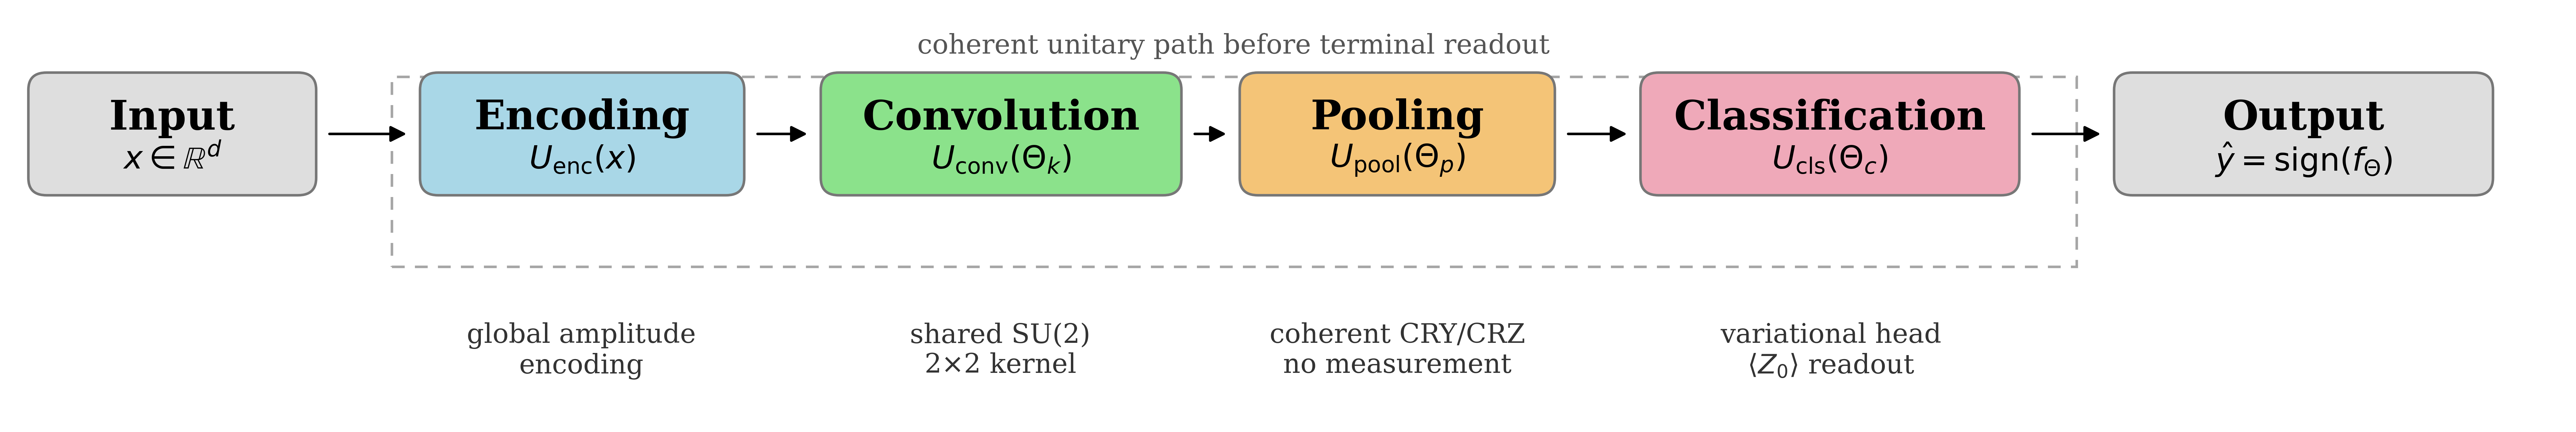
\includegraphics[width=\textwidth]{figs_final/fig1.png}
\caption{Overall FQCNN architecture. The pipeline runs Input $\rightarrow$ Encoding $\rightarrow$ Convolution $\rightarrow$ Pooling $\rightarrow$ Classification $\rightarrow$ Output. Every stage operates through unitary quantum operations, with no intermediate measurements.}
\label{fig:arch}
\end{figure*}

\section{Related Work}
\subsection{Quantum Convolutional Neural Networks}
Quantum convolutional neural networks extend classical convolutional networks into the quantum domain by combining local unitary operations with hierarchical dimensionality reduction. The canonical QCNN uses a structured variational circuit inspired by renormalisation techniques~\cite{ref37}, while hierarchical quantum classifiers provide a related tree-like construction~\cite{ref46}.  In particular, measurement-based pooling requires a mid-circuit measurement and classical feed-forward, whereas the proposed block keeps the register coherent until the terminal observable~\cite{ref37}.

\subsection{Variational Quantum Classifiers and Trainability}
The broader framework of variational quantum circuits (VQCs) underlies most quantum machine learning models~\cite{ref40}. Optimisation commonly uses gradient-based updates and stochastic variants~\cite{ref15,ref21}. Increasing circuit depth and expressibility does not always help; it can produce barren plateaus, where gradient magnitudes become small as system size grows~\cite{ref14,ref19,ref38}. Strategies based on structured ansatz design and cost-function-aware optimisation can soften these effects~\cite{ref47}. These observations motivate empirical trainability checks for each proposed architecture.

\subsection{Quantum Autoencoders and Information Compression}
Dimensionality reduction in quantum models is often expressed through quantum autoencoder frameworks, which compress quantum states into lower-dimensional subspaces while preserving relevant information~\cite{ref25,ref26}. Recent work also studies information compression with structured quantum autoencoders~\cite{ref23}. Autoencoders offer a principled route to quantum information compression, but they typically require separate encoding--decoding stages. By contrast, embedded pooling mechanisms that operate directly within QCNN architectures provide an alternative path to information reduction.

\subsection{Noise and Error Mitigation in Quantum Learning}
Noise remains a primary obstacle to deploying quantum machine learning models on near-term hardware. Comprehensive reviews of quantum error mitigation cover strategies such as zero-noise extrapolation, data-driven correction, and probabilistic error cancellation~\cite{ref22}. Recent work also studies data-augmented learning for noise mitigation~\cite{ref16}. These methods operate at the error-mitigation or training layer; the present work instead treats architectural noise behaviour as a specified finite-simulation question.

\section{Evaluation Questions and Evidence Boundaries}
The evaluation is organised around four questions that separate an
architectural identity from an empirical performance claim. This separation is
important for a fully coherent model: a circuit can remove a dynamic-control
requirement without improving accuracy, and an accuracy result can be useful as
a benchmark without establishing a quantum advantage. The questions are
therefore evaluated with different units of evidence rather than collapsed into
one score.

\begin{table*}[!t]
\caption{Evaluation questions, evidence layers, and the corresponding claim boundary. The table distinguishes exact statements about the implemented circuit from finite empirical observations.}
\label{tab:questions}
\centering
\small
\begin{tabular}{@{}p{0.19\textwidth}p{0.25\textwidth}p{0.25\textwidth}p{0.23\textwidth}@{}}
\toprule
\textbf{Question} & \textbf{Operational test} & \textbf{Evidence used} & \textbf{Interpretation permitted} \\
\midrule
Does the main path remain coherent? & Inspect the circuit operations and terminal measurement; verify that intermediate operations are unitary. & Circuit operation audit and state-purity check. & A property of the implementation; not a hardware execution claim. \\
Does coherent pooling reproduce the compared channel? & Compare the controlled unitary followed by a partial trace with the explicitly constructed measure-and-condition channel. & Theorem~\ref{thm:exact}, numerical channel comparison, and dephasing controls. & Exact equivalence for the stated block, with no claim that information or accuracy is recovered. \\
How does the model behave empirically? & Use fixed binary tasks, common ordered samples, common data splits, five seeds, and one final test evaluation. & Four-task primary aggregate, same-split logistic/MLP/TTN baselines, uncertainty, and paired tests. & A finite within-study comparison; no state-of-the-art or quantum-advantage claim. \\
What limits practical interpretation? & Audit effective capacity, finite-size gradients, expressibility, information dynamics, noise sensitivity, and logical/transpiled resources. & Model-analysis diagnostics and local Qiskit transpilation and noise simulations. & Bounded simulator and local-transpilation observations; no asymptotic or device-performance guarantee. \\
\bottomrule
\end{tabular}
\end{table*}

\subsection{From architectural identity to empirical estimands}
The first two questions are principally mathematical. The statement that the
main path is unitary follows from the operation types in the executed tape, and
the pooling statement follows from the controlled-unitary factorisation proved
in Section~\ref{sec:pooling-theory}. Their numerical checks are evaluated at the reference checkpoint (Section~\ref{sec:reference})
rather than as estimates of a population.


The performance question has a different estimand. For task $d$ and model arm
$m$, let $A_{d,m,s}$ be the accuracy on the final test partition for seed $s$.
The reported point estimate is the mean over the seed set,
\begin{equation}
\begin{aligned}
\bar{A}_{d,m}&=\frac{1}{S}\sum_{s=1}^{S}A_{d,m,s},\\
s_{d,m}&=\left[\frac{1}{S}\sum_{s=1}^{S}
\left(A_{d,m,s}-\bar{A}_{d,m}\right)^2\right]^{1/2}.
\end{aligned}
\label{eq:seedestimand}
\end{equation}
where $S=5$ in the primary matrix. The standard deviation in the tables is the
population standard deviation of these five runs.
For a comparator $c$, the paired effect is computed seed by seed as
$\Delta_{d,c,s}=A_{d,\mathrm{FQCNN},s}-A_{d,c,s}$. This makes the split and seed
the unit of the primary comparison and keeps per-example tests in a descriptive
role.

The third question asks where the fixed architecture sits relative to transparent baselines under one reproducible protocol. The model has a globally amplitude-encoded input and only ten qubits, while the classical baselines see the original 784 flattened features, so the comparison controls the data, splits, seeds, and validation-only selection rule rather than parameter count or computational cost.

\subsection{Negative findings}
We report the negative findings alongside the positive ones: the FQCNN is below
the logistic and dense baselines on all four primary tasks, the wider coherent
and SU(4) pooling families do not automatically improve the proposed
construction, and the full dynamical Lie algebra rules out a polynomial-size
trainability certificate. A non-significant paired test with five seeds is not
interpreted as equivalence, and local fake-backend transpilation is not treated
as hardware validation.

\section{Proposed FQCNN Architecture}
\subsection{Design requirements and register notation}
The architecture is designed around four requirements. First, all trainable
transformations after state preparation must be expressible as quantum gates
with a single terminal observable. Second, the convolutional kernel must be
shared across its register-index windows so that parameter allocation is
independent of the number of windows. Third, pooling must reduce the active
register without inserting a measurement or a classical branch. Fourth, the
implementation must expose enough structure to audit dead parameter slots,
discarded wires, and resource costs separately.

Let $A_0=\{0,\ldots,n-1\}$ denote the active wires immediately after state
preparation. At pooling stage $\ell$, the executed pairing is
$P_\ell=\{(a_i,b_i)\}_{i=1}^{m_\ell}$, where $a_i$ is retained and $b_i$ is
compressed. The retained and compressed sets are
$R_\ell=\{a_i\}$ and $C_\ell=\{b_i\}$. If the active-register cardinality is
odd, the final unpaired wire is collected in $O_\ell$ and retired at the same
stage. Writing $U_\ell$ for the convolution and pooling operations emitted at
that stage, the state passed to the next active register is represented by
\begin{equation}
\rho_{\ell+1}=\operatorname{Tr}_{C_\ell\cup O_\ell}
\!\left[U_\ell\rho_\ell U_\ell^{\dagger}\right],
\qquad A_{\ell+1}=R_\ell.
\label{eq:active-register}
\end{equation}
Equation~\eqref{eq:active-register} is a description of the reduced state on
the wires used later; the full state remains pure before the inactive wires are
ignored. No reset is inserted into the circuit. The partial trace is
the mathematical description of the fact that a retired wire is not addressed
by later gates or the terminal observable.

\begin{table*}[!t]
\caption{Executed register schedules and parameter allocation used by the finite-size audits. ``Allocated'' includes slots reserved by the model layout; ``effective'' counts slots with a gradient magnitude above $10^{-12}$ in the corresponding finite diagnostic.}
\label{tab:schedule}
\centering
\small
\begin{tabular}{@{}rccccc@{}}
\toprule
\textbf{$n$} & \textbf{Input geometry} & \textbf{Active-wire schedule} & \textbf{Pooling stages} & \textbf{Allocated slots} & \textbf{Effective slots} \\
\midrule
4 & $4\times4$ & $4\rightarrow2\rightarrow1$ & 2 & 188 & 62 \\
6 & $8\times8$ & $6\rightarrow3\rightarrow1$ & 2 & 194 & 62 \\
8 & $16\times16$ & $8\rightarrow4\rightarrow2\rightarrow1$ & 3 & 260 & 122 \\
10 & $28\times28$ & $10\rightarrow5\rightarrow2\rightarrow1$ & 3 & 269 & 74 \\
\bottomrule
\end{tabular}
\end{table*}

The ten-qubit schedule is not a conventional square image lattice after the
first reduction: ten wires become five, then two, then one. The convolutional
window generator therefore operates on the current active-index arrangement,
whereas the input itself remains a global amplitude state. We therefore use the term ``register-index window'' throughout.

\subsection{Problem Formulation}
Consider a labelled dataset $\mathcal{D} = \{(x^{(k)}, y^{(k)})\}$ for $k = 1, \ldots, N$ in a supervised setting, where $x \in \mathbb{R}^d$ is the input feature vector, $x_i \in [-1, 1]$, $y \in \{-1, 1\}$, and $d$ is the number of features after preprocessing. To scale efficiently, we use amplitude encoding, which maps the input vector into a quantum state. We consider a register of $n = 10$ qubits all initialised in the ground state
\begin{equation}
|\psi_0\rangle = |0\rangle^{\otimes 10}.
\end{equation}
A two-dimensional input image $X \in \mathbb{R}^{28 \times 28}$ is flattened into a 784-dimensional vector $x$, which is zero-padded to 1024 and mapped to the $2^{10} = 1024$ state amplitudes using global amplitude encoding. The full model is a parameterised unitary circuit built from the following operations:
\begin{equation}
U(\Theta; x) = U_{\text{cls}}(\theta_c)\, U_{\text{pool}}(\theta_p)\, U_{\text{conv}}(\theta_k)\, U_{\text{enc}}(x),
\end{equation}
where $\Theta = \{\theta_c, \theta_p, \theta_k\}$. The scalar model output is defined as
\begin{equation}
f_\theta(x) = \langle\psi_0|U^\dagger(\Theta; x)\, Z_0\, U(\Theta; x)|\psi_0\rangle,
\end{equation}
and classification is performed via
\begin{equation}
\hat{y}(x) = \text{sign}\big(f_\theta(x)\big).
\end{equation}
All intermediate transformations are strictly unitary, with no mid-circuit measurements.

\subsection{Quantum Data Encoding}
\label{sec:encoding}
The implementation uses one state-preparation operation: global amplitude encoding. It maps a normalised classical input vector into the amplitudes of a ten-qubit state, representing up to $2^{10}$ features without introducing a second data-dependent feature map. Prior to encoding, each input feature is min-max normalised to the bounded domain $[a, b] = [0, 1]$:
\begin{equation}
x_i' = \frac{x_i - x_{\min}}{x_{\max} - x_{\min}} \cdot (b - a) + a, \qquad [a, b] = [0, 1].
\end{equation}
The preprocessed vector is padded with zeros to length $2^{10}$ and prepared as
\begin{equation}
\begin{aligned}
|\psi_{\mathrm{enc}}(x)\rangle
 &= \operatorname{AmplitudeEmbedding}(x',\,\mathrm{wires}=0{:}9,\\
 &\quad \mathrm{normalize}=\mathrm{true},\,\mathrm{pad}=0)\,|0\rangle^{\otimes 10}.
\end{aligned}
\end{equation}
No per-qubit rotations or data-dependent ring-correlation gates are applied on top of this operation in the main amplitude-encoded path. Consequently, the locality statements below refer to the support and parameter sharing of variational gates in the register-index space, not to spatially adjacent pixels in the original image.

\subsection{Quantum Convolutional Layer}
The convolutional layer applies a parameter-shared variational kernel over all 2$\times$2 sliding windows. The complete pipeline is summarised in Fig.~\ref{fig:arch}; the circuit-level kernel used in each window is shown in Fig.~\ref{fig:kernel}.

\subsubsection{Kernel parameterisation}
Let each window contain four qubits. For a kernel depth $d$ and depth slice $k$, the single-qubit rotation block is
\begin{equation}
V_q^{(k)}(\Theta_k) = R_X\!\big(\theta_{X,q}^{(k)}\big) R_Z\!\big(\theta_{Z,q}^{(k)}\big) R_Y\!\big(\theta_{Y,q}^{(k)}\big).
\end{equation}
Each qubit is parameterised using full SU(2) rotations in the selected ansatz while keeping the circuit shallow. Here $\Theta_k \in \mathbb{R}^{4 \times d \times 3}$, so $|\Theta_k| = 12d$. Parameter sharing enforces $\Theta_k(\omega) = \Theta_k$ for all register-index windows $\omega$, so the parameter count does not grow with the number of windows. 

\subsubsection{Intra-window entanglement}
Within each window, entanglement is introduced through the unitary
\begin{align}
U_{\text{ent}}(\omega) = {}&\text{CNOT}_{q_1 \rightarrow q_2}\, \text{CNOT}_{q_0 \rightarrow q_3}\, \text{CNOT}_{q_1 \rightarrow q_3} \notag\\
&\times\, \text{CNOT}_{q_0 \rightarrow q_2}\, \text{CNOT}_{q_2 \rightarrow q_3}\, \text{CNOT}_{q_0 \rightarrow q_1},
\end{align}
with the rightmost operator acting first. The six gates couple every pair of qubits in the register-index window. This all-to-all pattern provides bounded gate support at a fixed depth, while entanglement does not cross a window boundary.  The full convolution operator is
\begin{equation}
U_{\text{conv}}(\Theta_k) = \prod_{\omega} U_{\text{ent}}(\omega)\, V_\omega(\Theta_k).
\end{equation}

\begin{figure}[!t]
\centering
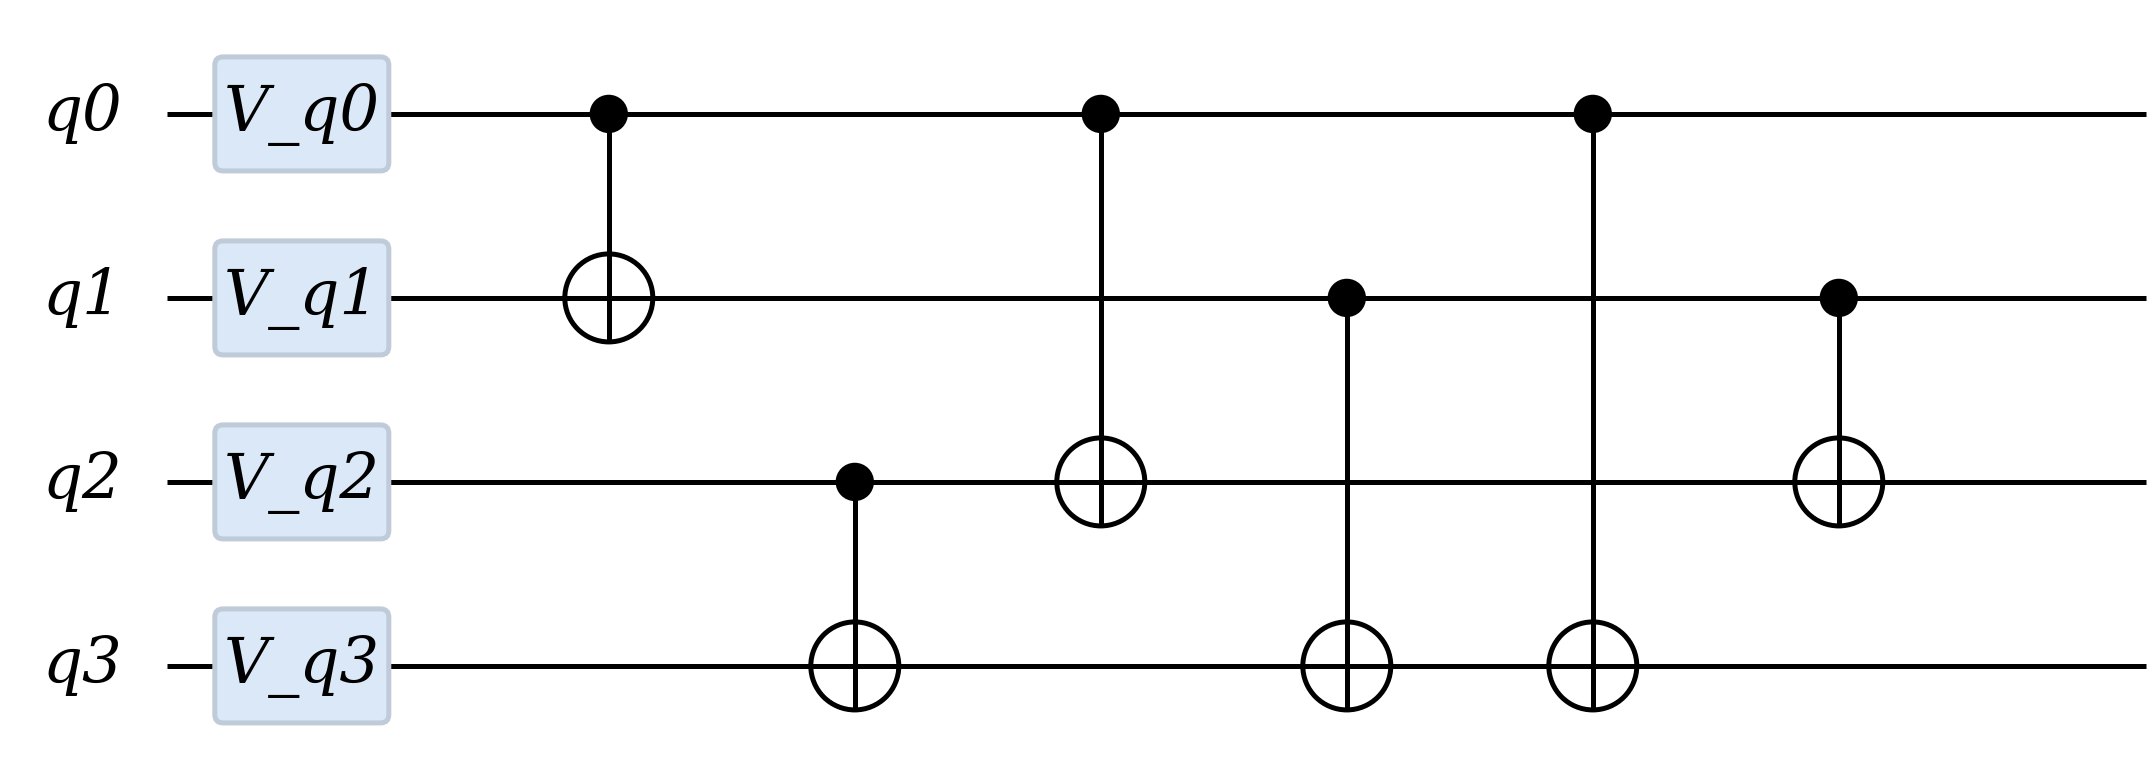
\includegraphics[width=\columnwidth]{figs_final/fig3.png}
\caption{The 2$\times$2 register-index convolutional kernel acting on window $\omega = \{q_0, q_1, q_2, q_3\}$. The gates $V_q$ apply full SU(2) rotations per qubit with parameters shared across all register-index windows.  The six CNOTs realise all-to-all entanglement inside the window.}
\label{fig:kernel}
\end{figure}

\subsection{Coherence-Preserving Pooling}
\subsubsection{Pooling pair set}
After convolution, the qubits are grouped into disjoint ordered pairs as illustrated in Fig.~\ref{fig:pooling}.
\begin{equation}
P \subseteq \big\{(a, b) \mid a, b \in \{1, \ldots, N\},\ a \neq b\big\}.
\end{equation}
Each pair $(a, b) \in P$ designates $a$ as the retained qubit and $b$ as the compressed qubit, with pairs mutually disjoint:
\begin{equation}
(a, b), (c, d) \in P \Rightarrow \{a, b\} \cap \{c, d\} = \varnothing.
\end{equation}

\subsubsection{Pooling unitary}
For every pair $(a, b) \in P$, with the compressed qubit $b$ acting as control and the retained qubit $a$ as target, we apply
\begin{equation}
W_{ab}(\Theta_p) = R_Y^{(a)}(\gamma_{ab})\, R_Y^{(b)}(\epsilon)\, \text{CRZ}_{b \to a}(\beta_{ab})\, \text{CRY}_{b \to a}(\alpha_{ab}),
\label{eq:poolblock}
\end{equation}
where operators act right to left and $\epsilon = 0.02$ is a fixed (non-trainable) angle applied to the compressed qubit. Because $b$ is excluded from all subsequent operations, $R_Y^{(b)}(\epsilon)$ has no effect on any observable of the retained register; it is kept so that the parameter vector matches the implemented model. Section~\ref{sec:pooling-theory} makes this inertness precise. The global pooling operator is
\begin{equation}
U_{\text{pool}}(\Theta_p) = \prod_{(a,b) \in P} W_{ab}(\Theta_p).
\end{equation}
The control assignment in~\eqref{eq:poolblock} is not incidental: both two-qubit gates are diagonal in the computational basis of the compressed qubit $b$, which is the structural property Section~\ref{sec:pooling-theory} rests on.

\subsubsection{Dimensional reduction}
After pooling, only the retained qubits $a$ stay active; the compressed qubits $b$ are discarded after the unitary evolution. At a stage with $N$ active wires, the executed pair-and-retire schedule forms $m=|P|=\lfloor N/2\rfloor$ consecutive pairs and retires any unpaired wire. Thus the active output count is $n_r=m$ (rather than $N-m$ when $N$ is odd), and the pooling parameter count is $|\Theta_p|=3|P|$. For the ten-qubit model the active-wire schedule is $10\rightarrow5\rightarrow2\rightarrow1$. The pooling therefore performs structured dimensionality reduction while preserving the pre-discard global state as a pure state.

\begin{figure}[!t]
\centering
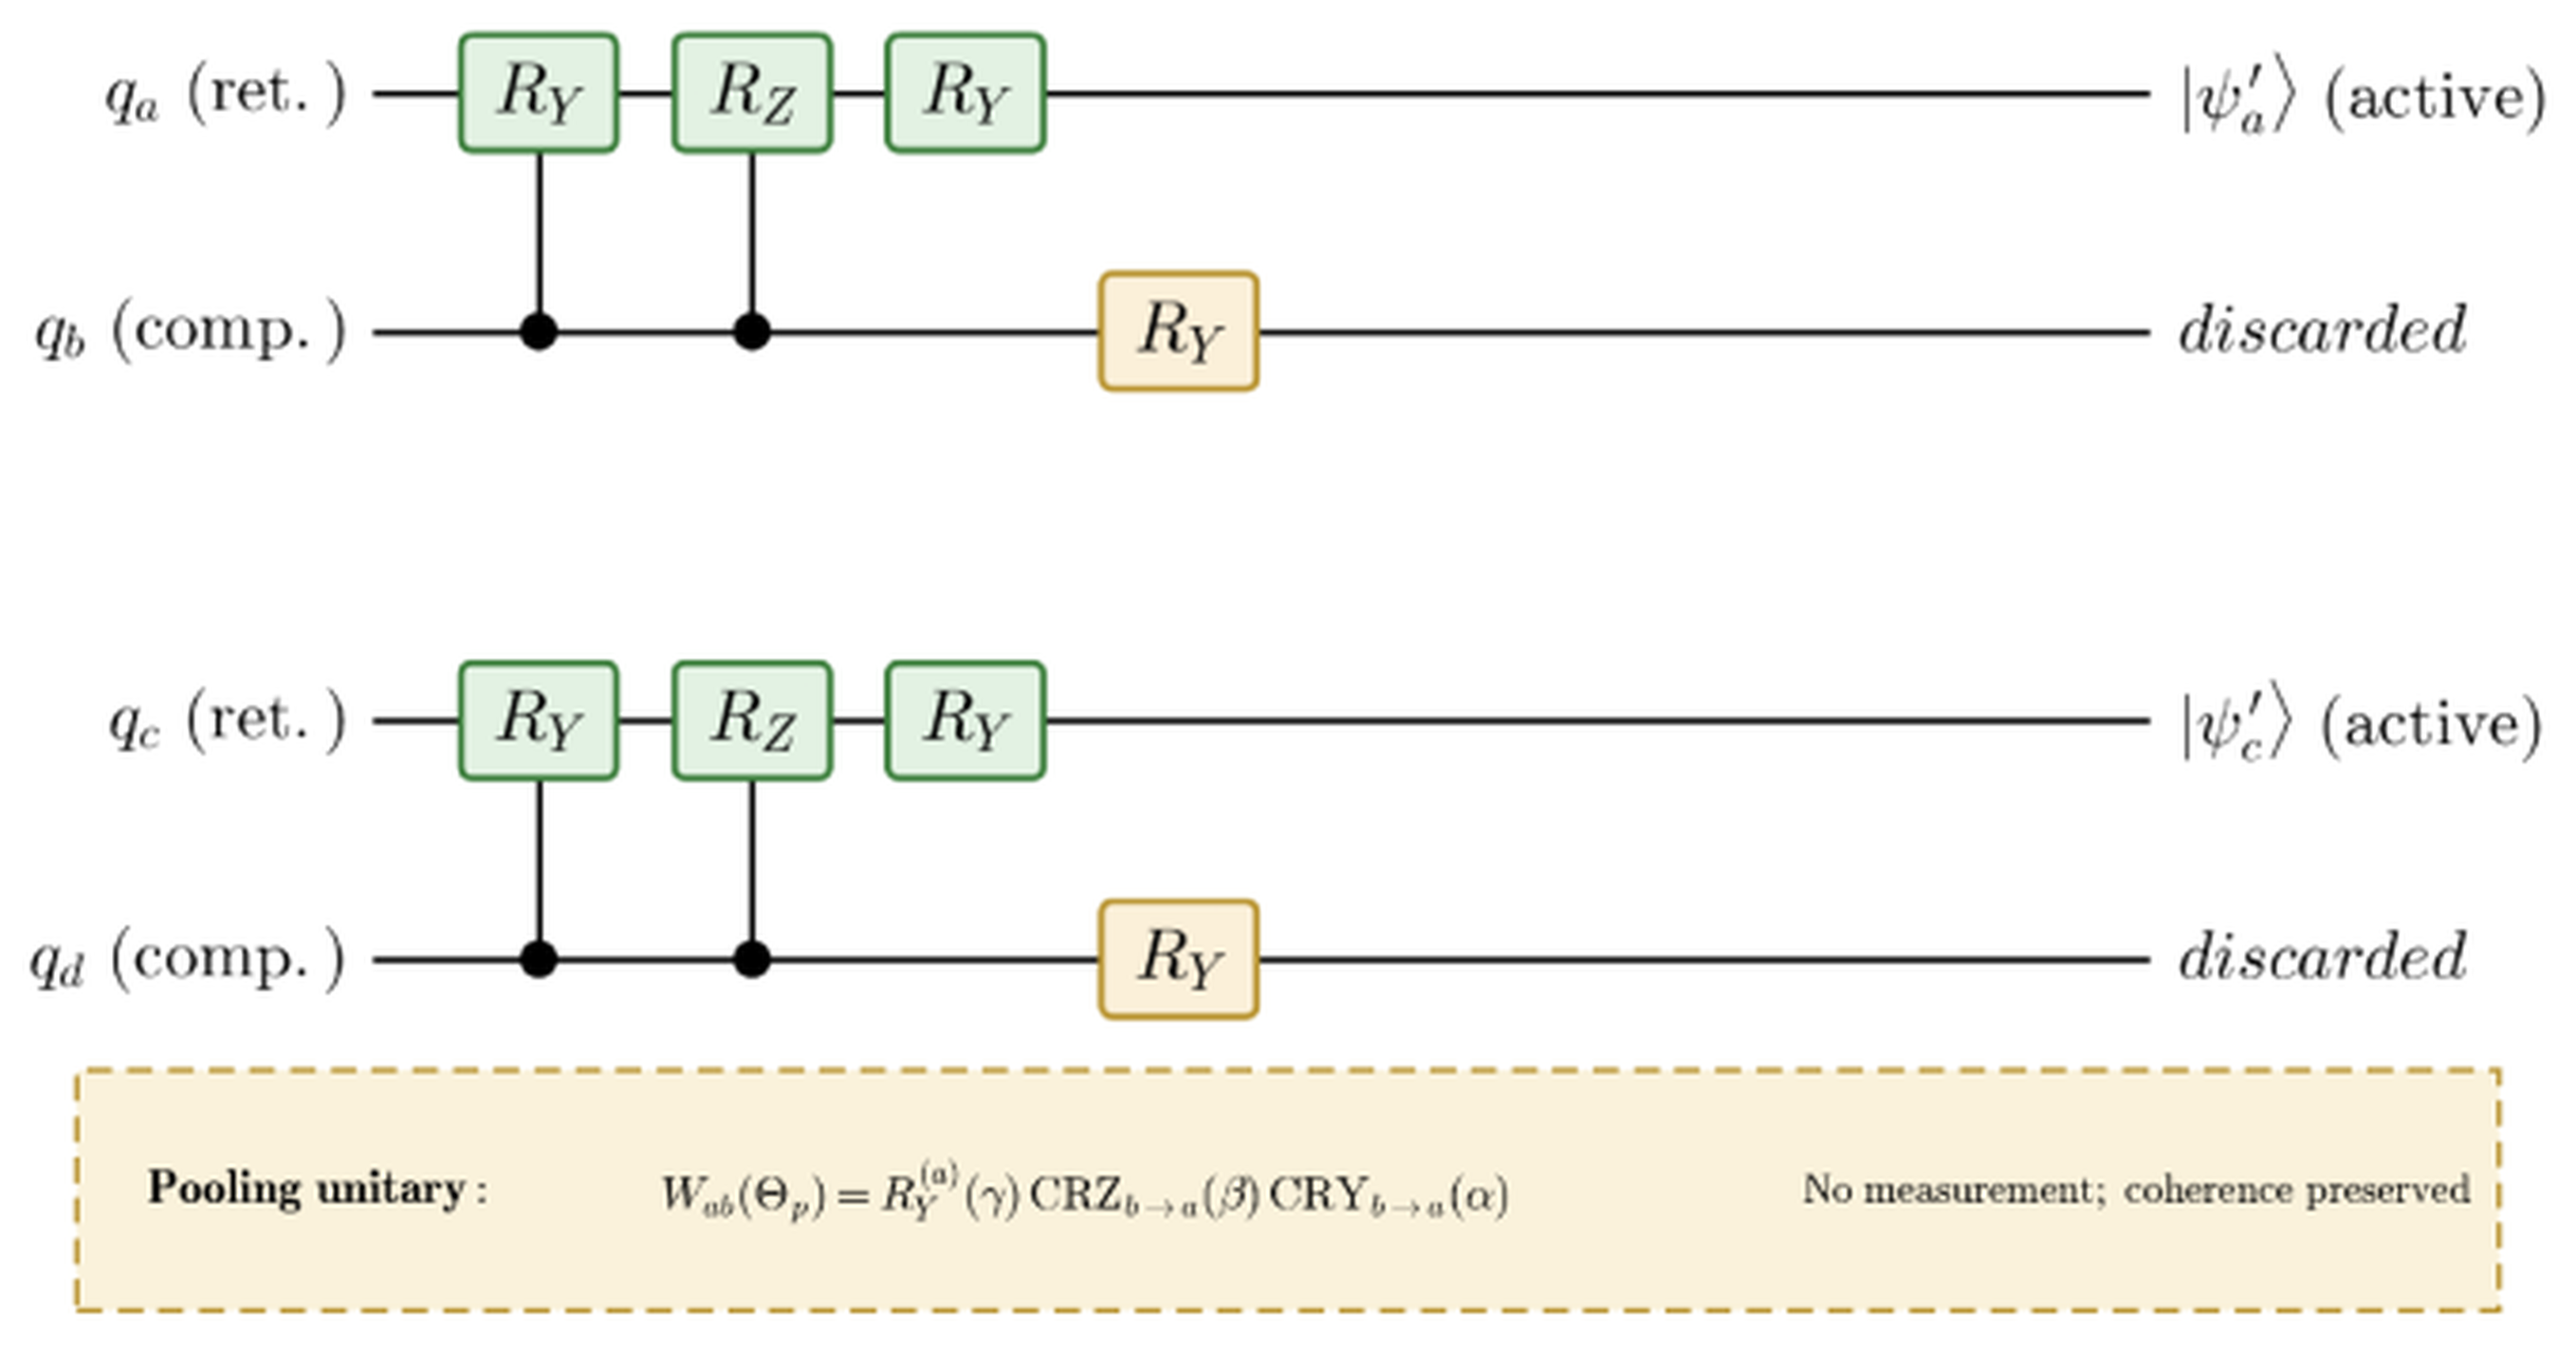
\includegraphics[width=\columnwidth]{figs_final/fig4.png}
\caption{Coherent unitary pooling mechanism. For each disjoint pair $(a, b) \in P$, qubit $a$ is retained and $b$ is compressed. The unitary $W_{ab}$ transfers information from $q_b$ into $q_a$ via CRY and CRZ gates \emph{controlled on $q_b$} and targeting $q_a$, followed by a local $R_Y$ on each wire, with no mid-circuit measurement. The compressed qubit is excluded from all later operations; any unpaired wire is also retired by the executed schedule, while the global state remains pure before the active-register reduction.}
\label{fig:pooling}
\end{figure}

\subsection{Unitary Versus Measurement-Based Pooling}
\label{sec:pooling-theory}

A measurement-based QCNN pooling block can measure the compressed qubit and apply a classically conditioned correction to the retained qubit. The construction here instead uses a coherent two-qubit unitary. This section establishes the exact relationship between those two specified blocks: the block in~\eqref{eq:poolblock} \emph{reproduces} the stated measurement-based channel exactly, without requiring mid-circuit measurement, qubit reset, or classical feed-forward.

\subsubsection{Setup}
Fix a pair $(a,b) \in P$ and let $\rho$ be the joint state of $(a,b)$ immediately before pooling. A \emph{measure-and-condition} pooling step measures $b$ in the computational basis and, on outcome $m \in \{0,1\}$, applies $U_m \in SU(2)$ to $a$. Averaged over outcomes, the retained register undergoes the channel
\begin{equation}
\mathcal{M}_{\{U_m\}}(\rho) = \sum_{m \in \{0,1\}} U_m \, \langle m |_b \rho | m \rangle_b \, U_m^{\dagger}.
\label{eq:mcchannel}
\end{equation}

\begin{theorem}[Exact simulation]
\label{thm:exact}
Let $U_0 = R_Y(\gamma_{ab})$ and $U_1 = R_Y(\gamma_{ab}) R_Z(\beta_{ab}) R_Y(\alpha_{ab})$. Then for every input state $\rho$,
\begin{equation}
\mathrm{Tr}_b\!\left[ W_{ab} \rho\, W_{ab}^{\dagger} \right] = \mathcal{M}_{\{U_0, U_1\}}(\rho).
\end{equation}
That is, the coherent block in~\eqref{eq:poolblock} induces exactly the measure-and-condition channel~\eqref{eq:mcchannel} on the retained register, and therefore reproduces every observable statistic of measurement-based pooling.
\end{theorem}

\begin{proof}
Both two-qubit gates in~\eqref{eq:poolblock} are controlled on $b$, hence diagonal in $b$'s computational basis:
\begin{equation}
\text{CRZ}_{b \to a}(\beta)\,\text{CRY}_{b \to a}(\alpha) = \sum_{m} |m\rangle\langle m|_b \otimes V_m,
\end{equation}
with $V_0 = I$ and $V_1 = R_Z(\beta) R_Y(\alpha)$. The local $R_Y^{(a)}(\gamma)$ commutes with every projector on $b$, so absorbing it gives $|m\rangle\langle m|_b \otimes U_m$ with $U_m = R_Y(\gamma) V_m$, matching the statement. Writing $V = \sum_m |m\rangle\langle m|_b \otimes U_m$ we have $W_{ab} = \big(R_Y^{(b)}(\epsilon) \otimes I_a\big) V$, and since the partial trace over $b$ is invariant under any unitary acting on $b$ alone,
\begin{equation}
\mathrm{Tr}_b\!\left[W_{ab} \rho W_{ab}^{\dagger}\right] = \mathrm{Tr}_b\!\left[V \rho V^{\dagger}\right] = \sum_m U_m \langle m|_b \rho |m\rangle_b U_m^{\dagger}. \qedhere
\end{equation}
\end{proof}

The same result can be written in Kraus form, which makes the deferred
measurement interpretation explicit. Define
\begin{equation}
K_m=U_m\,{}_b\!\langle m|,\qquad m\in\{0,1\}.
\label{eq:pool-kraus}
\end{equation}
The operators map the joint pair to the retained subsystem and satisfy
$\sum_m K_m^{\dagger}K_m=I_a\otimes I_b$. Hence
$\mathcal{M}_{\{U_m\}}(\rho)=\sum_mK_m\rho K_m^{\dagger}$ is a completely
positive trace-preserving map. The coherent implementation replaces the
classical record $m$ with the computational-basis value already present in
the control wire. Tracing that wire at the end of the pooling block produces
the same Kraus sum because the partial trace contracts the two copies of
$|m\rangle\langle m|$ and removes cross terms between distinct outcomes.

This derivation also identifies the exact boundary of the result. The
compressed wire's off-diagonal blocks are not used by the controlled block,
so they cannot influence the retained output after tracing out that wire. A
general two-qubit unitary need not have this property: it can rotate the
compressed subsystem before the reduction and thereby make its coherences
operationally visible. The strict-containment proposition is therefore a
statement about the available channel family, not a claim that the
three-angle block exploits its whole family.

Theorem~\ref{thm:exact} gives a direct deferred-measurement construction for the stated pooling channel. Three consequences follow, each true of the executed model:
\begin{enumerate}
\item Coherent pooling \emph{loses nothing} relative to measurement-based pooling for the retained-register channel; it simulates that class without mid-circuit control.
\item It does so while eliminating mid-circuit measurement, qubit reset, and classical feed-forward --- capabilities that may require additional control support on a target device. 
\item The global state remains pure from state preparation to the single terminal measurement, and the circuit is differentiable end to end (here by backpropagation).
\end{enumerate}

It also follows immediately that $R_Y^{(b)}(\epsilon)$ in~\eqref{eq:poolblock} is inert: it acts only on $b$, and the partial trace over $b$ absorbs it. This is an analytic invariant of the stated retained-register channel, independent of the fixed angle's numerical value.

\begin{proposition}[Strict containment]
\label{prop:containment}
The family of unitary pooling channels $\{\rho \mapsto \mathrm{Tr}_b[V \rho V^{\dagger}] : V \in SU(4)\}$ \emph{strictly} contains the measure-and-condition class $\{\mathcal{M}_{\{U_m\}}\}$.
\end{proposition}

\begin{proof}
Containment is Theorem~\ref{thm:exact} applied to $V = \sum_m |m\rangle\langle m|_b \otimes U_m$. For strictness, take $V = e^{i\pi/4}\mathrm{SWAP} \in SU(4)$. Its global phase cancels from the channel, so $\mathrm{Tr}_b[V \rho V^{\dagger}] = \rho_b$, the full reduced state of $b$ including its off-diagonal elements. By contrast, $\mathcal{M}_{\{U_m\}}$ depends on $b$ only through the diagonal blocks $\langle m|_b \rho |m\rangle_b$. The product states $\rho_a \otimes |{+}\rangle\langle{+}|_b$ and $\rho_a \otimes \tfrac{1}{2}I_b$ have identical $b$-diagonals and are therefore indistinguishable to every $\mathcal{M}_{\{U_m\}}$, yet $V$ maps them to $|{+}\rangle\langle{+}|$ and $\tfrac{1}{2}I$ respectively, which are at trace distance $\tfrac{1}{2}$.
\end{proof}

Proposition~\ref{prop:containment} places the proposed block precisely: it realises the measurement-simulable subclass in the proposed construction, while the strict extension --- non-diagonal $V$ --- represents headroom that is an empirical question rather than an architectural claim.

\begin{proposition}[Coherence-transfer functional]
\label{prop:coh}
Let $\mathcal{D}_b$ be complete dephasing of $b$ in the computational basis and define
\begin{equation}
\Delta_{\mathrm{coh}}(V) = \big\| \mathrm{Tr}_b[V \rho V^{\dagger}] - \mathrm{Tr}_b[V \mathcal{D}_b(\rho) V^{\dagger}] \big\|_1 .
\label{eq:cohfunctional}
\end{equation}
Then $\Delta_{\mathrm{coh}}(W_{ab}) = 0$ for every $\rho$, whereas $\Delta_{\mathrm{coh}}(e^{i\pi/4}\mathrm{SWAP}) > 0$.
\end{proposition}

\begin{proof}
By Theorem~\ref{thm:exact} the output of $W_{ab}$ depends on $\rho$ only through $\langle m|_b \rho |m\rangle_b$, which $\mathcal{D}_b$ leaves invariant; hence the two terms coincide. For $e^{i\pi/4}\mathrm{SWAP}$ the witness in Proposition~\ref{prop:containment} gives $\Delta_{\mathrm{coh}} = 1$ on $\rho_a \otimes |{+}\rangle\langle{+}|_b$ under the trace-norm definition in~\eqref{eq:cohfunctional}; the corresponding trace distance is $\tfrac{1}{2}$.
\end{proof}

\subsubsection{Numerical confirmation}
The analytic statements are also checked on the executed circuit. Evaluating the $n=10$ reference checkpoint (Section~\ref{sec:reference}) on a density-matrix simulator, the coherent block and the explicit measure-and-condition channel of~\eqref{eq:mcchannel} produce terminal expectation values agreeing to a maximum deviation of $2.2 \times 10^{-16}$ --- floating-point round-off, against a tolerance of $10^{-12}$. Independently, inserting complete dephasing on every compressed wire immediately before pooling, at unchanged parameters, changes the readout by at most $5.86 \times 10^{-14}$ and leaves the predicted class unchanged for all eight evaluated inputs, so the observed accuracy difference on this check is zero. The retained-wire dephasing control changes the readout by $0.4094$, confirming that the null effect is specific to the compressed subsystem and its partial trace.

\subsubsection{Scope of the result}
Theorem~\ref{thm:exact} does not imply that the coherent block preserves
retained-register information that the measurement-based block destroys: for
observables of this circuit, the two channels are identical. It establishes
exact simulation of the measurement-based class without mid-circuit
measurement, reset, or feed-forward, a globally pure state throughout the
pipeline, and end-to-end differentiability. Whether the strict
extension of Proposition~\ref{prop:containment} yields an accuracy benefit is
tested by the pooling ablation in Section~\ref{sec:results}.

\subsection{Variational Classification Head}
The classification head maps the compressed representation to a Pauli-$Z$ expectation on the first active wire. Its description follows the executed circuit rather than a simplified symbolic surrogate. On each of at most the first four active wires $q_i$, it applies $R_X(\theta_{2i})$, $R_Y(\theta_{2i+1})$, and $R_Z(\theta_{2i+8})$ in sequence. A nearest-neighbour CNOT chain with a wraparound CNOT is followed by $R_X(\theta_{2i+16})$ and $R_Y(\theta_{2i+17})$ on those wires, then one additional CNOT from the first to the second active wire when at least two remain. The implementation allocates a 32-slot classifier vector and uses modular indexing so the same layout applies across supported register sizes.

A final $R_Z(\theta_{31})$ is syntactically applied to the readout wire immediately before measuring $Z$. Because this gate commutes with the measured observable, it cannot change the expectation and has exactly zero gradient; it is kept only to preserve the implemented parameter layout and is not a trainable bias. For the ten-qubit circuit, there are 269 allocated parameter slots, 78 slots that reach the tape, and 74 effective slots at the declared $|\partial f/\partial\theta|>10^{-12}$ tolerance. The distinction matters because unused convolutional arrays, unpaired wires, and structurally inert gates leave allocated slots that do not influence the terminal observable.

\subsection{Global Parameter Scaling}
Parameter sharing prevents the number of allocated slots from scaling with the number of windows, but the executed topology determines which slots are used. We therefore report allocated, tape-reaching, and effective counts separately rather than applying a closed-form count that assumes every module is independently instantiated.

\subsection{Capacity accounting and executed-tape audit}
\label{sec:capacity}
The parameter vector is intentionally larger than the set of values that
influence the terminal observable. Each of the four convolutional arrays is
allocated as a $4\times4\times3$ tensor, giving 48 slots per layer. Three
pooling arrays reserve five three-angle pairs each, and the classifier reserves
32 slots. The ten-qubit layout therefore allocates
$4(48)+3(5\times3)+32=269$ slots. The executed active-wire schedule addresses
only a subset of the nominal convolutional windows, and the classifier uses
modular indexing; these implementation details make a single nominal
parameter-count number misleading.

\begin{table*}[!t]
\caption{Capacity and operation accounting for the ten-qubit circuit. The rows answer different questions and are not interchangeable.}
\label{tab:capacity}
\centering
\small
\begin{tabular}{@{}p{0.31\textwidth}r p{0.55\textwidth}@{}}
\toprule
\textbf{Quantity} & \textbf{Value} & \textbf{Definition} \\
\midrule
Allocated parameter slots & 269 & Reserved by the model layout \\
Tape-reaching slots & 78 & Slots syntactically read by the executed tape \\
Effective slots & 74 & $|\partial f/\partial\theta|>10^{-12}$ audit \\
Trainable gates on tape & 222 & Parameterised gate occurrences \\
Gates driven by effective slots & 218 & Occurrences from the 74 live slots \\
Total tape operations & 327 & Trainable and fixed operations \\
\bottomrule
\end{tabular}
\end{table*}

The gate count used in the capacity
scaling diagnostic is 222, not 74: 48 effective slots are reused across more
than one gate occurrence, with up to four occurrences driven by one slot. The
two counts thus differ in opposite directions. The audit was performed both on
the reference checkpoint over 20 fixed inputs and in the
independent random-initialisation gradient sweep described in
Section~\ref{sec:diagnostics}; the two audits give the same effective count.

The same distinction matters for classical simulation. At ten qubits, the
statevector has $2^{10}=1024$ complex amplitudes and is directly tractable on a
classical computer. The small state space and shallow executed tape are the
reasons every result in this paper can be checked exactly or with explicitly
declared finite-shot local simulation.  In particular, the resource counts below separate
state preparation from the model body so that the cost of loading a classical
image is not hidden behind the variational circuit.

\subsection{Architectural Interpretation}
The FQCNN implements global amplitude state preparation, shared register-index convolutional mixing, coherent dimensional compression, and variational classification before a terminal Pauli-$Z$ expectation. Its effective capacity is described by the executed-tape and gradient audits above; no expressive benefit is attributed to the inert terminal $R_Z$.

\section{Training and Optimization}
\subsection{Learning Objective and Risk Functional}
The learning objective is governed by empirical risk minimisation. The model maps the quantum expectation value $f_\Theta(x^{(k)})$ to a bounded probability and maps labels to $\tilde{y}^{(k)} \in \{0,1\}$:
\begin{equation}
p^{(k)} = \frac{\operatorname{clip}\!\left(f_\Theta(x^{(k)}),-1,1\right) + 1}{2}.
\end{equation}
The executed class-weighted Binary Cross-Entropy (BCE) objective is
\begin{equation}
\begin{aligned}
\mathcal{L}(\Theta) = -\frac{1}{M} \sum_{k=1}^{M} \Big[&w_{+}\tilde{y}^{(k)} \log\!\big(p^{(k)}+\varepsilon\big) \\
&+ w_{-}\big(1 - \tilde{y}^{(k)}\big) \log\!\big(1 - p^{(k)}+\varepsilon\big)\Big],
\end{aligned}
\end{equation}
where $M$ is the mini-batch size, $w_{+}$ and $w_{-}$ are computed from the training split only, and $\varepsilon=10^{-7}$ prevents singular logarithms. This is a weighted Bernoulli negative log-likelihood.

\subsection{Measurement Estimation Model}
On hardware the expectation value is estimated through repeated measurements. With $S$ shots, the estimator is
\begin{equation}
\hat{f}_\theta(x) = \frac{1}{S} \sum_{n=1}^{S} z^{(n)}, \qquad z^{(n)} \in \{-1, +1\}.
\end{equation}
It satisfies $\mathbb{E}[\hat{f}_\theta] = f_\theta$ and $\text{Var}[\hat{f}_\theta] = (1 - f_\theta^2)/S$, so the estimator is unbiased and its variance decreases as $\mathcal{O}(1/S)$.

\subsection{Gradient Evaluation}
The reported statevector training uses backpropagation on PennyLane's \texttt{default.qubit} simulator. For a hardware implementation, gates with a two-eigenvalue generator admit an exact occurrence-level parameter-shift estimator; this is included only as a cost model and is not the differentiation method used for the reported results. In the interior of the clipping interval, the executed BCE formulation gives
\begin{align}
\frac{\partial \mathcal{L}}{\partial \theta} = -\frac{1}{2M} \sum_{k=1}^{M}
\left[\frac{w_{+}\tilde{y}^{(k)}}{p^{(k)}+\varepsilon}
-\frac{w_{-}(1-\tilde{y}^{(k)})}{1-p^{(k)}+\varepsilon}\right]
\frac{\partial f_{\Theta}(x^{(k)})}{\partial \theta}.
\end{align}
where, for one eligible gate occurrence $j$, $\partial f/\partial\theta_j = \tfrac{1}{2}(f_{j,+}-f_{j,-})$ with shifts $\pm\pi/2$. If one trainable slot is reused in $r$ gate occurrences, the chain rule sums those occurrence-level derivatives, requiring up to $2r$ shifted circuit evaluations absent a specialised grouped rule. 

\subsection{Optimization Procedure}
The optimisation loop uses the Adam optimiser with mini-batches of $M = 32$, gradient clipping to norm 5, and an Exponential Moving Average (EMA) of the parameters with decay 0.99. After every epoch the EMA parameters are scored on the validation partition, and the checkpoint with the highest validation accuracy is kept. After three epochs without improvement the learning rate is halved; training stops when it would fall below $10^{-4}$ or when the epoch limit is reached. The full settings are listed in Table~\ref{tab:training}.

\subsection{Reference checkpoint for circuit diagnostics}
\label{sec:reference}
The circuit-level diagnostics in Sections~\ref{sec:pooling-theory},
\ref{sec:capacity}, and~\ref{sec:infodyn} use one reference checkpoint of the
ten-qubit model. It was
trained with the procedure above on the full stratified MNIST 0-vs-1 split
(7,599 training and 1,900 validation images; seed 42; learning rate 0.005; at
most 50 epochs) and reached 98.2\% validation accuracy. It is used only to fix
concrete parameter values for these diagnostics; the accuracy comparison uses
the per-seed checkpoints of Section~\ref{sec:results}.

\subsection{Reproducible training protocol}
The comparison campaign treats data identity, split identity, model selection,
and test evaluation as separate objects. The protocol is summarised in
Algorithm~\ref{alg:protocol}.

\begin{algorithm}[!t]
\caption{Training and evaluation protocol}
\label{alg:protocol}
\begin{algorithmic}[1]
\STATE Select a dataset family and binary class pair from the task list.
\STATE Load the source dataset and assign stable sample IDs.
\STATE Form the 666-example task pool and create a deterministic stratified 60/15/25 split.
\STATE Apply the fixed preprocessing and amplitude encoding.
\FOR{each arm and seed}
  \STATE Initialise the arm with the given seed and fixed configuration.
  \STATE Train on the training partition only; score the EMA parameters on the validation partition after each epoch.
  \STATE Restore the validation-selected checkpoint.
  \STATE Evaluate the test partition once and record the predictions and metrics.
\ENDFOR
\STATE Aggregate the per-seed test results for each task and arm.
\STATE Compute seed-level uncertainty and paired tests.
\end{algorithmic}
\end{algorithm}

Rounding the 60/15/25 fractions of the 666-example pool gives 400 training,
100 validation, and 166 test examples. The sample pool is selected before any
test evaluation and the same ordered identifiers are supplied to every arm. A
test label is never used for checkpoint selection, early stopping, or
hyperparameter choice.

\begin{table*}[!t]
\caption{Protocol controls for the within-study comparison.}
\label{tab:protocol-controls}
\centering
\small
\begin{tabular}{@{}p{0.20\textwidth}p{0.34\textwidth}p{0.34\textwidth}@{}}
\toprule
\textbf{Control} & \textbf{Implementation} & \textbf{Reason for reporting it} \\
\midrule
Task definition & Four binary tasks are fixed in advance: MNIST 0-vs-1, MNIST 3-vs-5, Fashion-MNIST 0-vs-6, and KMNIST 2-vs-3. & Covers an easy calibration task, a harder in-domain pair, and two further dataset families, and avoids post hoc task selection. \\
Split identity & Each seed uses a stored stratified split with stable sample IDs. & Ensures that every arm is trained and tested on the same partition. \\
Model selection & Validation accuracy selects the checkpoint and drives the learning-rate schedule; the test partition is read once at the end. & Prevents test-driven selection and keeps the final metric attached to the selected checkpoint. \\
Capacity disclosure & FQCNN allocation, tape usage, effective slots, logistic coefficients, and MLP parameters are reported separately. & Avoids calling the two-unit MLP parameter-matched when its dense parameter count is larger. \\
Seed aggregation & Five seeds are paired by task and split; population standard deviation and seeded bootstrap intervals are reported. & Displays training variability and avoids treating individual test examples as independent repetitions of training. \\
\bottomrule
\end{tabular}
\end{table*}

The main simulator path uses PennyLane's \texttt{default.qubit} backpropagation
device for batched training and retains \texttt{lightning.qubit} as a sequential
correctness oracle. A separate regression suite verifies agreement of outputs,
losses, all 269 parameter gradients, and one Adam update between the two paths,
which are built from the same circuit definition.

The local preprocessing function min--max normalises the image matrix to
$[0,1]$, flattens each native $28\times28$ image, pads it with zeros to 1024
entries, and maps the two source labels to $-1$ and $+1$. The amplitude embedding
then performs the per-state $\ell_2$ normalisation required by state preparation.
 This is a fixed preprocessing step, not a learned feature-extraction stage.

\subsection{Computational Complexity}
For the simulator path, backpropagation cost is determined by the retained state and circuit evaluation rather than by parameter-shift executions. If parameter-shift is used on hardware, its leading evaluation count is two shifted circuits per eligible gate occurrence and datapoint, with additional accounting for reused slots and shot cost set by the measurement budget. Statevector simulation scales as $\mathcal{O}(2^n)$ in memory. 

\subsection{Noise and Gradient Stability}
\subsubsection{Statistical measurement noise}
With $\rho(\Theta; x) = |\psi(\Theta; x)\rangle\langle\psi(\Theta; x)|$ and Born's rule, $f_\theta(x) = \text{Tr}[\rho Z_0]$. Each shifted expectation estimator is unbiased with variance scaling as $\mathcal{O}(1/S)$, so their linear parameter-shift estimate of $\partial f/\partial\theta$ is unbiased. A finite-shot plug-in estimator of the Binary Cross-Entropy gradient need not be unbiased, however, because the loss is nonlinear in the estimated probability and requires clipping near 0 and 1.

\subsubsection{Hardware-induced quantum noise}
Hardware noise replaces unitary evolution with a completely positive trace-preserving map $\rho_{\text{noisy}} = \varepsilon(\rho)$. Under the stated global depolarising model $\varepsilon_{\text{dep}}(\rho) = (1 - p)\rho + p\, I/2^n$, a traceless Pauli-$Z$ expectation is attenuated by $(1-p)$. Under the phase-flip model $\varepsilon_{\text{phase}}(\rho) = (1 - p)\rho + p Z\rho Z$, computational-basis off-diagonal terms are rescaled according to the affected wire. Section~\ref{sec:noise} evaluates these channels in simulation.

\subsubsection{Noise propagation}
Entangling operations have bounded support in the register-index topology, but global amplitude encoding prevents this fact from being interpreted as a bound on image-space noise propagation. End-to-end noisy accuracy is therefore measured empirically in Section~\ref{sec:noise}.

\subsubsection{Effect on gradients}
If the noise channel is independent of $\theta$, differentiation moves inside the trace, $\partial f/\partial\theta = \text{Tr}[\varepsilon(\partial\rho/\partial\theta)Z_0]$. The resulting gradient behavior depends on the channel and circuit.

\section{Experimental Results and Analysis}
\subsection{Dataset Description}
We evaluate four binary tasks drawn from three $28\times28$ grayscale dataset families: the MNIST handwritten-digit dataset~\cite{ref49} (digits 0-vs-1 and 3-vs-5), Fashion-MNIST (T-shirt/top vs Shirt), and Kuzushiji-MNIST (classes 2-vs-3). Each task uses 666 examples with a stratified 60/15/25 split for every seed, validation-only model selection, and exactly one final test evaluation per seed. Table~\ref{tab:q1data} summarises the tasks.

\begin{table*}[!t]
\caption{Evaluation tasks. Each task uses 666 source examples and a stratified 400/100/166 train/validation/test split for seeds 0--4.}
\label{tab:q1data}
\centering
\begin{tabular}{@{}lllll@{}}
\toprule
\textbf{Task} & \textbf{Dataset/classes} & \textbf{Role} & \textbf{Split} & \textbf{Seeds} \\
\midrule
MNIST 0-vs-1 & MNIST (0, 1) & calibration & 400/100/166 & 0--4 \\
MNIST 3-vs-5 & MNIST (3, 5) & harder in-domain & 400/100/166 & 0--4 \\
Fashion 0-vs-6 & Fashion-MNIST (T-shirt/top, Shirt) & cross-domain clothing & 400/100/166 & 0--4 \\
KMNIST 2-vs-3 & Kuzushiji-MNIST (2, 3) & distinct script domain & 400/100/166 & 0--4 \\
\bottomrule
\end{tabular}
\end{table*}

Each input is min-max normalised to [0, 1], flattened to 784 values, zero-padded to 1024, and embedded directly into one ten-qubit state by global amplitude encoding.  Labels are mapped to $\{+1, -1\}$ for the Pauli-$Z$ expectation output. MNIST 0-vs-1 serves as an easy calibration task, MNIST 3-vs-5 as a harder in-domain pair, and Fashion-MNIST and KMNIST as two further dataset families.

\subsection{Experimental Setup and Training Configuration}
All experiments use numerical quantum simulation on a register of $n = 10$ qubits initialised in $|0\rangle^{\otimes 10}$, with the amplitude-encoded input described in Section~\ref{sec:encoding}. Training and evaluation use PennyLane's \texttt{default.qubit} exact statevector simulator with backpropagation. The model comprises convolutional layers with shared SU(2) kernels, coherence-preserving pooling layers, and a final variational classification head. Training uses mini-batch optimisation with Adam, gradient clipping, and EMA of parameters. The exact training settings are listed in Table~\ref{tab:training}.

\begin{table}[!t]
\caption{Training configuration for the primary comparison.}
\label{tab:training}
\centering
\begin{tabular}{ll}
\toprule
\textbf{Parameter} & \textbf{Value} \\
\midrule
Epochs & 30 maximum \\
LR schedule & halve after 3 epochs without improvement \\
Gradient clipping & norm 5 \\
EMA decay & 0.99 \\
Batch size & 32 \\
Learning rate & 0.02 \\
Optimizer & Adam \\
Loss function & Weighted Binary Cross-Entropy \\
Quantum device & default.qubit (PennyLane, backprop) \\
Shots & None (exact statevector) \\
Seeds & 0, 1, 2, 3, 4 \\
Per-task split & 400 / 100 / 166 (train / validation / test) \\
\bottomrule
\end{tabular}
\end{table}

\subsection{Results}
\label{sec:results}

For each task and arm, accuracy is summarised across the five seed-level test
evaluations by its mean and population standard deviation. The primary paired
test uses the five per-seed accuracies in a two-sided Wilcoxon signed-rank test;
the twelve task--comparator tests are corrected as one Holm--Bonferroni family at
$\alpha=0.05$. The reported 95\% intervals are seeded percentile bootstrap
intervals for the mean using 10,000 resamples. Exact McNemar tests are used only
as descriptive per-seed diagnostics on paired correctness vectors; no pooled
McNemar p-value is used for confirmatory inference. With five paired seeds, these
tests have limited power, so non-significance is not interpreted as equivalence.

\subsection{Analysis of Model Performance}
The unitary construction preserves the global state until the terminal observable, and the pooling theorem establishes exact equivalence to the corresponding measure-and-condition channel for the stated block. The empirical contribution is assessed by the primary aggregate, pooling-transfer ablation, finite-size diagnostics, and local resource and noise simulations.

\subsection{Comparison with Existing QCNN Approaches}

\begin{table}[!t]
\caption{Comparison arms. Pool: pooling type (U = unitary); Coh.: fully coherent circuit; Params: trainable parameters (allocated/effective for FQCNN). TTN denotes the balanced tree tensor network of Grant et al.~\cite{ref46}.}
\label{tab:comparison}
\centering
\begin{tabular}{@{}lccc@{}}
\toprule
\textbf{Method} & \textbf{Pool} & \textbf{Coh.} & \textbf{Params} \\
\midrule
FQCNN (ours) & U & Yes & 269/74 \\
Logistic & -- & -- & 785 \\
MLP (2-unit) & -- & -- & 1,573 \\
TTN & U & Yes & 48 \\
\bottomrule
\end{tabular}
\end{table}

\begin{table*}[!t]
\caption{Test accuracy of all arms (mean $\pm$ standard deviation over five seeds). All arms use the same ordered samples, data split, and single final test evaluation.}
\label{tab:q1comparison}
\centering
\begin{tabular}{lcccc}
\toprule
\textbf{Task} & \textbf{FQCNN} & \textbf{Logistic} & \textbf{MLP} & \textbf{TTN} \\
\midrule
Fashion 0-vs-6 &  0.789 $\pm$ 0.019 & 0.842 $\pm$ 0.014 & 0.824 $\pm$ 0.015 & 0.787 $\pm$ 0.073 \\
KMNIST 2-vs-3 &  0.884 $\pm$ 0.023 & 0.947 $\pm$ 0.024 & 0.933 $\pm$ 0.016 & 0.867 $\pm$ 0.062 \\
MNIST 0-vs-1 &  0.975 $\pm$ 0.013 & 0.995 $\pm$ 0.005 & 0.988 $\pm$ 0.009 & 0.961 $\pm$ 0.016 \\
MNIST 3-vs-5 &  0.800 $\pm$ 0.030 & 0.948 $\pm$ 0.012 & 0.877 $\pm$ 0.044 & 0.730 $\pm$ 0.047 \\
\bottomrule
\end{tabular}
\end{table*}

\begin{table*}[!t]
\caption{Test metrics for FQCNN (mean $\pm$ population standard deviation over five seeds).}
\label{tab:q1metrics}
\centering
\begin{tabular}{lccccc}
\toprule
\textbf{Task} & \textbf{Accuracy} & \textbf{Balanced acc.} & \textbf{F1} & \textbf{ROC-AUC} & \textbf{PR-AUC} \\
\midrule
Fashion 0-vs-6 &  0.789 $\pm$ 0.019 & 0.789 $\pm$ 0.019 & 0.784 $\pm$ 0.021 & 0.863 $\pm$ 0.017 & 0.842 $\pm$ 0.045 \\
KMNIST 2-vs-3 &  0.884 $\pm$ 0.023 & 0.884 $\pm$ 0.023 & 0.893 $\pm$ 0.020 & 0.968 $\pm$ 0.005 & 0.969 $\pm$ 0.003 \\
MNIST 0-vs-1 &  0.975 $\pm$ 0.013 & 0.975 $\pm$ 0.013 & 0.975 $\pm$ 0.013 & 0.997 $\pm$ 0.002 & 0.998 $\pm$ 0.002 \\
MNIST 3-vs-5 &  0.800 $\pm$ 0.030 & 0.800 $\pm$ 0.030 & 0.776 $\pm$ 0.033 & 0.901 $\pm$ 0.035 & 0.896 $\pm$ 0.040 \\
\bottomrule
\end{tabular}
\end{table*}

\begin{table*}[!t]
\caption{Per-seed accuracy values underlying the primary comparison. The seed order is 0, 1, 2, 3, 4 for every column; values are shown to four decimal places to make the seed-level pairing visible.}
\label{tab:seedvalues}
\centering
\small
\begin{tabular}{@{}llrrrrr@{}}
\toprule
\textbf{Task} & \textbf{Arm} & \textbf{Seed 0} & \textbf{Seed 1} & \textbf{Seed 2} & \textbf{Seed 3} & \textbf{Seed 4} \\
\midrule
Fashion 0-vs-6 & FQCNN & 0.8072 & 0.7952 & 0.8072 & 0.7771 & 0.7590 \\
 & Logistic & 0.8313 & 0.8614 & 0.8373 & 0.8554 & 0.8253 \\
 & MLP & 0.8072 & 0.8434 & 0.8253 & 0.8373 & 0.8072 \\
 & TTN & 0.8072 & 0.8012 & 0.8313 & 0.8494 & 0.6446 \\
\addlinespace
KMNIST 2-vs-3 & FQCNN & 0.8855 & 0.8554 & 0.9036 & 0.9157 & 0.8614 \\
 & Logistic & 0.9819 & 0.9096 & 0.9578 & 0.9458 & 0.9398 \\
 & MLP & 0.9518 & 0.9157 & 0.9518 & 0.9277 & 0.9157 \\
 & TTN & 0.9277 & 0.7892 & 0.9096 & 0.9157 & 0.7952 \\
\addlinespace
MNIST 0-vs-1 & FQCNN & 0.9759 & 0.9639 & 0.9578 & 0.9819 & 0.9940 \\
 & Logistic & 1.0000 & 0.9880 & 0.9940 & 0.9940 & 1.0000 \\
 & MLP & 0.9940 & 0.9819 & 0.9880 & 0.9759 & 1.0000 \\
 & TTN & 0.9819 & 0.9578 & 0.9699 & 0.9337 & 0.9639 \\
\addlinespace
MNIST 3-vs-5 & FQCNN & 0.7651 & 0.8133 & 0.7771 & 0.7952 & 0.8494 \\
 & Logistic & 0.9398 & 0.9337 & 0.9518 & 0.9458 & 0.9699 \\
 & MLP & 0.8675 & 0.8795 & 0.9036 & 0.8012 & 0.9337 \\
 & TTN & 0.7651 & 0.7470 & 0.6386 & 0.7590 & 0.7410 \\
\bottomrule
\end{tabular}
\end{table*}

\begin{table*}[!t]
\caption{Seed-level paired effects for the primary comparison. Each entry is FQCNN accuracy minus comparator accuracy, followed by the unadjusted and Holm-adjusted two-sided Wilcoxon $p$ values. The twelve tests form one Holm family.}
\label{tab:pairedeffects}
\centering
\small
\begin{tabular}{@{}lccc@{}}
\toprule
\textbf{Task} & \textbf{FQCNN $-$ Logistic} & \textbf{FQCNN $-$ MLP} & \textbf{FQCNN $-$ TTN} \\
\midrule
Fashion-MNIST 0-vs-6 & $-0.0530$; $p=.0625$, $p_H=.7500$ & $-0.0349$; $p=.0656$, $p_H=.7500$ & $+0.0024$; $p=.7150$, $p_H=1.0000$ \\
KMNIST 2-vs-3 & $-0.0627$; $p=.0625$, $p_H=.7500$ & $-0.0482$; $p=.0625$, $p_H=.7500$ & $+0.0169$; $p=.4652$, $p_H=1.0000$ \\
MNIST 0-vs-1 & $-0.0205$; $p=.0625$, $p_H=.7500$ & $-0.0133$; $p=.1250$, $p_H=.7500$ & $+0.0133$; $p=.6250$, $p_H=1.0000$ \\
MNIST 3-vs-5 & $-0.1482$; $p=.0625$, $p_H=.7500$ & $-0.0771$; $p=.0625$, $p_H=.7500$ & $+0.0699$; $p=.0679$, $p_H=.7500$ \\
\bottomrule
\end{tabular}
\end{table*}

\begin{figure}[!t]
\centering
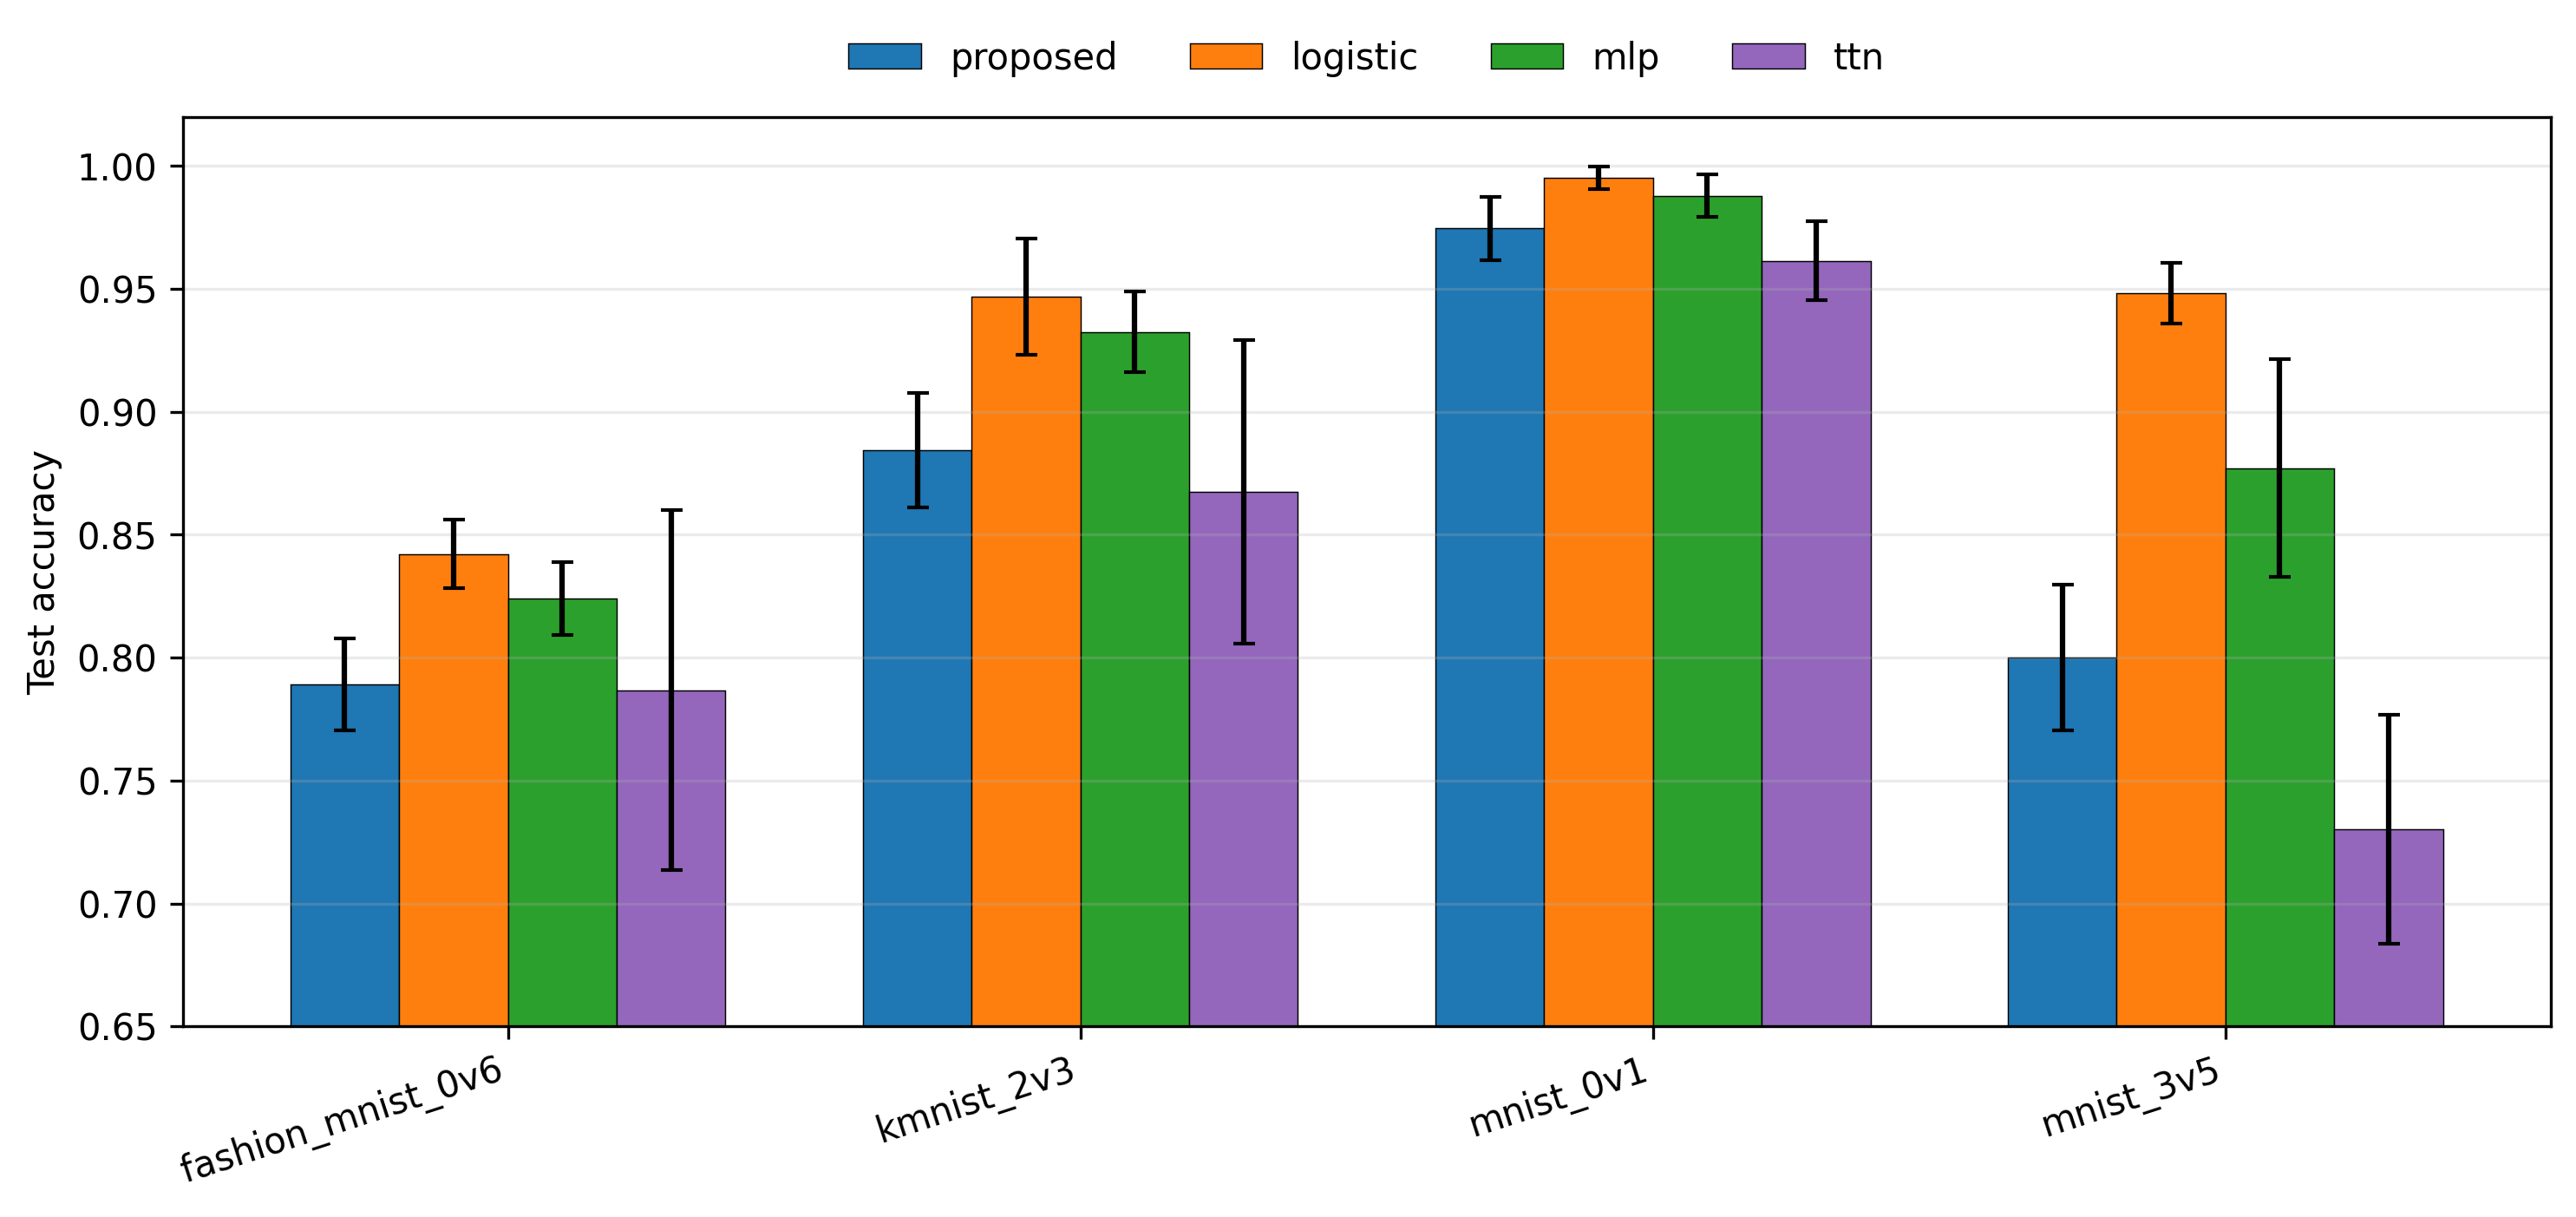
\includegraphics[width=\columnwidth]{figs_final/q1_comparison.png}
\caption{Test accuracy of all arms on the four tasks (mean $\pm$ standard deviation over five seeds).}
\label{fig:q1comparison}
\end{figure}

The primary comparison is within-study: logistic regression, a compact two-unit dense MLP, and the balanced tree tensor network (TTN) of Grant et al.~\cite{ref46} are evaluated on the same ordered samples, data splits, and seed set as the FQCNN. The arm definitions and parameter accounting are given in Table~\ref{tab:comparison}. The logistic model has 785 trainable coefficients for the 784 flattened pixels, the two-unit MLP has 1,573 dense parameters, and the ten-qubit TTN has 48 trainable parameters under the executed consecutive-pair tree schedule. The MLP is therefore not parameter-matched to the FQCNN's 269 allocated/74 effective quantum slots. Table~\ref{tab:q1comparison} and Fig.~\ref{fig:q1comparison} show the accuracy result, while Table~\ref{tab:q1metrics} reports the FQCNN metric vector. The FQCNN is below logistic regression and the MLP on all four tasks, while exceeding TTN on all four in mean accuracy (paired tests in Table~\ref{tab:pairedeffects}).

\subsubsection{Cross-task interpretation}
The per-seed values in Table~\ref{tab:seedvalues} show why the seed distribution is
more informative than a single headline score. On MNIST 0-vs-1, every arm is
strong and the FQCNN reaches $0.975\pm0.013$, so the task mainly serves as a
calibration check. The harder MNIST 3-vs-5 task
separates the hierarchical quantum arm from the linear baseline: FQCNN accuracy
is $0.800\pm0.030$, TTN is $0.730\pm0.047$, and the logistic baseline is
$0.948\pm0.012$. The FQCNN thus exceeds TTN in mean accuracy here but remains well below logistic regression.

The cross-domain tasks expose a different pattern. FQCNN reaches
$0.789\pm0.019$ on Fashion-MNIST 0-vs-6 and $0.884\pm0.023$ on KMNIST 2-vs-3,
while logistic regression remains higher on both. The TTN variance is notably
larger on Fashion-MNIST ($0.073$ versus $0.019$ for FQCNN), whereas the mean
accuracies are nearly tied. On KMNIST, FQCNN exceeds TTN by roughly two
percentage points in mean accuracy, again without a multiplicity-adjusted
significant paired effect. Overall, the FQCNN's performance relative to the baselines depends strongly on the task.

Table~\ref{tab:pairedeffects} shows the paired effects. The
FQCNN--logistic and FQCNN--MLP effects are negative for every task, and the
FQCNN--TTN effects are positive for every task. Nevertheless, the five-seed
Wilcoxon tests do not survive the Holm correction. 

\begin{table}[!t]
\caption{Pooling-transfer ablation on Fashion-MNIST 0-vs-6 (three seeds). Holm-adjusted $p$ values are two-sided seed-level Wilcoxon tests versus the unitary reference over four variants.}
\label{tab:pooling-transfer}
\centering
\begin{tabular}{@{}lcc@{}}
\toprule
\textbf{Pooling variant} & \textbf{Accuracy} & \textbf{$p_{\mathrm{Holm}}$} \\
\midrule
Unitary (reference) & 0.803 $\pm$ 0.006 & -- \\
No pooling & 0.815 $\pm$ 0.006 & 0.719 \\
Measurement & 0.803 $\pm$ 0.006 & 1.000 \\
Coherent & 0.791 $\pm$ 0.023 & 1.000 \\
SU(4) & 0.801 $\pm$ 0.013 & 1.000 \\
\bottomrule
\end{tabular}
\end{table}

The transfer experiment in Table~\ref{tab:pooling-transfer} uses the same 166-example test set and clean checkpoints for seeds 0--2. No variant differs from the unitary reference after Holm correction, although three seeds give little statistical power.

\subsection{Secondary pooling-family evidence}
A separate pooling-arm experiment provides a complementary, smaller-budget
view of the pooling family. It used the ten-qubit geometry, a 571-example pool per task split 343/86/142 (train/validation/test), 30 epochs, five seeds, and three binary MNIST tasks. Because its task set and split sizes differ from
the four-task comparison, it is reported separately and is not merged into the
primary results.

\begin{table*}[!t]
\caption{Secondary pooling-arm comparison. Entries are test accuracy means $\pm$ population standard deviation over five seeds for each task. Each arm has 15 cells in total (three tasks and five seeds).}
\label{tab:secondary-pooling}
\centering
\small
\begin{tabular}{@{}lccccc@{}}
\toprule
\textbf{Task} & \textbf{No pooling} & \textbf{Measurement} & \textbf{Unitary} & \textbf{Coherent} & \textbf{SU(4)} \\
\midrule
MNIST 0-vs-1 & $0.9507\pm0.0134$ & $0.9662\pm0.0082$ & $0.9662\pm0.0082$ & $0.9634\pm0.0113$ & $0.9718\pm0.0161$ \\
MNIST 3-vs-5 & $0.7620\pm0.0376$ & $0.8070\pm0.0440$ & $0.8070\pm0.0440$ & $0.8099\pm0.0134$ & $0.8634\pm0.0451$ \\
MNIST 4-vs-9 & $0.8394\pm0.0113$ & $0.8606\pm0.0233$ & $0.8606\pm0.0233$ & $0.8662\pm0.0461$ & $0.8704\pm0.0580$ \\
\bottomrule
\end{tabular}
\end{table*}

Across these secondary tasks, removing pooling lowers the aggregate mean by
2.7 percentage points relative to the unitary arm and is significant in the
paired tests. The measurement and unitary rows tie exactly in the
statevector implementation, as expected from the theorem and deferred
measurement. The coherent extension improves the aggregate by only 0.19
percentage points and is not significant. The SU(4) arm has a 2.4 percentage
point aggregate advantage, with the largest task-level separation on
MNIST 3-vs-5; the seed-level Wilcoxon result does not confirm that advantage
after Holm correction. This suggests headroom within the wider pooling family; the three-angle block is not necessarily optimal.

\subsection{Information dynamics across the pooling cascade}
\label{sec:infodyn}
The word ``coherent'' can refer either to the purity of the complete state or to
the coherence of a reduced subsystem. These are not interchangeable. To make
the distinction observable, we recorded reduced-state diagnostics at the
encoded state, immediately before and after each pooling stage, and after the
classifier for eight inputs using the reference checkpoint. For a reduced density matrix
$\rho_A$, the reported $\ell_1$ coherence is
\begin{equation}
C_{\ell_1}(\rho_A)=\sum_{i\ne j}|(\rho_A)_{ij}|,
\end{equation}
and the entropy and mutual information are
{\scriptsize
\begin{equation}
S(\rho_A)=-\operatorname{Tr}(\rho_A\log_2\rho_A),\qquad
I(A:B)=S(\rho_A)+S(\rho_B)-S(\rho_{AB}).
\end{equation}
}
Purity is $\operatorname{Tr}(\rho_A^2)$. Entropies and mutual information in
Table~\ref{tab:information} are in bits; entries are mean $\pm$ standard
deviation over the eight inputs.

\begin{table*}[!t]
\caption{Per-stage information diagnostics for the ten-qubit reference checkpoint. The reduced state is taken on the active/kept wires; mutual information is reported only at pooling boundaries. }
\label{tab:information}
\centering
\small
\begin{tabular}{@{}lrrrrr@{}}
\toprule
\textbf{Stage} & \textbf{Kept wires} & \textbf{$C_{\ell_1}$} & \textbf{Purity} & \textbf{$S$} & \textbf{$I(\mathrm{keep}:\mathrm{discard})$} \\
\midrule
Encoded & 10 & $767.262\pm7.232$ & $1.0000\pm0.0000$ & $0.0000\pm0.0000$ & -- \\
Before pooling 0 & 5 & $5.906\pm0.206$ & $0.0919\pm0.0037$ & $3.9070\pm0.0321$ & $7.814\pm0.064$ \\
After pooling 0 & 5 & $6.567\pm0.170$ & $0.0942\pm0.0030$ & $3.8901\pm0.0309$ & $7.780\pm0.062$ \\
Before pooling 1 & 2 & $0.819\pm0.051$ & $0.3356\pm0.0051$ & $1.7565\pm0.0120$ & $0.204\pm0.009$ \\
After pooling 1 & 2 & $0.697\pm0.038$ & $0.3134\pm0.0044$ & $1.8214\pm0.0111$ & $0.358\pm0.013$ \\
Before pooling 2 & 1 & $0.403\pm0.017$ & $0.5923\pm0.0072$ & $0.8624\pm0.0111$ & $0.005\pm0.002$ \\
After pooling 2 & 1 & $0.332\pm0.022$ & $0.5879\pm0.0074$ & $0.8691\pm0.0114$ & $0.016\pm0.004$ \\
After classifier & 1 & $0.253\pm0.016$ & $0.5879\pm0.0074$ & $0.8691\pm0.0114$ & -- \\
\bottomrule
\end{tabular}
\end{table*}

The encoded ten-wire state has unit purity and near-zero entropy, as expected
for a pure state preparation. After tracing out the compressed wires, the
active reduced state is mixed because it is entangled with the inactive
subsystem; this is compatible with a globally pure unitary computation. By the
final readout, the one-wire reduced state has purity approximately $0.588$ and
entropy approximately $0.869$ bits, so ``fully coherent'' should not be read as
``locally pure'' or ``classically inaccessible.''

The mutual information falls from approximately $7.814$ bits before the first
pool to $0.204$ bits before the second and $0.005$ bits before the third. The
last pooling stage therefore has little measured keep--discard correlation on
these inputs. Pooling changes the entropy by less than $0.07$ bits at
each boundary, and the final classifier changes basis-dependent coherence
without changing the reduced state's spectrum. The controlled rotations provide a gate path for consolidating information, but the diagnostic does not show that each
pool concentrates useful information or that the deepest stage is active for
every task.

The dephasing controls of Section~\ref{sec:pooling-theory} ($0.4094$ on the
retained wires versus at most $5.86\times10^{-14}$ on the compressed wires)
are consistent with the theorem's specific subsystem statement and do not
imply that the discarded subsystem is irrelevant to the global state.

\subsection{Noise Robustness}
\label{sec:noise}
The pooling theorem and dephasing controls are circuit-level identities. To probe noise sensitivity we ran a bounded local noise experiment using trained checkpoints, depolarising and dephasing channels, fixed validation subsets, and the Qiskit Aer simulator. The protocol covers MNIST 3-vs-5 and Fashion-MNIST 0-vs-6, seeds 0--2, 25 validation samples per seed, noise levels $p\in\{0,0.005,0.01,0.02\}$, and 128 shots at nonzero levels; checkpoints are not retrained and the test split is never used. The zero-noise agreement check passes, while the finite-shot nonzero results vary across task, seed, channel, and level without a monotone pattern. 

\begin{table*}[!t]
\caption{Local noise-ladder validation accuracy averaged over three clean checkpoints and 25 validation examples per checkpoint. The zero-noise column is an exact statevector reference; nonzero columns use 128-shot local Aer simulation.  Checkpoints are not retrained.}
\label{tab:noise}
\centering
\small
\begin{tabular}{@{}llrrrr@{}}
\toprule
\textbf{Task} & \textbf{Channel} & \textbf{$p=0$} & \textbf{$p=0.005$} & \textbf{$p=0.01$} & \textbf{$p=0.02$} \\
\midrule
MNIST 3-vs-5 & Depolarising & 0.4400 & 0.4667 & 0.4933 & 0.5333 \\
 & Dephasing & 0.4400 & 0.5067 & 0.5067 & 0.4267 \\
Fashion-MNIST 0-vs-6 & Depolarising & 0.5867 & 0.4933 & 0.4667 & 0.4667 \\
 & Dephasing & 0.5867 & 0.5067 & 0.5333 & 0.4400 \\
\bottomrule
\end{tabular}
\end{table*}

The exact statevector and Aer statevector outputs agree at zero noise to a
maximum absolute difference below $1.34\times10^{-15}$ across the six
checkpoint records, confirming that the noise simulations start from the same
circuit as the noiseless model. With only 25 validation examples per checkpoint, a change in a few signs can move the accuracy by a large amount, so increasing $p$ need not produce a monotone sequence when the
checkpoint is fixed and shot noise is present.

\subsection{Scalability and Practicality}
Amplitude encoding fixes the state-vector width at the chosen qubit count, while parameter sharing controls the number of variational slots. Table~\ref{tab:resources} reports total logical, decomposed, and transpiled depths for $n=4,6,8,10$, including state preparation and readout. The transpilation target is the local Qiskit ``FakePeekskill'' BackendV2 with optimisation level 1 and a transpiler seed of 42; these are local resource estimates and no hardware was used.

\begin{table}[!t]
\caption{Total circuit-depth estimates from the local FakePeekskill transpilation audit.  Counts include state preparation, model body, and readout.}
\label{tab:resources}
\centering
\begin{tabular}{@{}rccc@{}}
\toprule
\textbf{$n$} & \textbf{Logical} & \textbf{Decomposed} & \textbf{Transpiled} \\
\midrule
4 & 38 & 73 & 343 \\
6 & 65 & 191 & 934 \\
8 & 113 & 626 & 2,549 \\
10 & 116 & 2,160 & 7,362 \\
\bottomrule
\end{tabular}
\end{table}

\begin{table*}[!t]
\caption{Pooling-arm practicality comparison at $n=4$ on the same local FakePeekskill BackendV2 target. Entries are depth/operation count at logical, decomposed, and transpiled levels.}
\label{tab:pooling-resources}
\centering
\small
\begin{tabular}{@{}lccccl@{}}
\toprule
\textbf{Arm} & \textbf{Mode} & \textbf{Logical} & \textbf{Decomposed} & \textbf{Transpiled} & \textbf{Control characteristic} \\
\midrule
No pooling & none & 30/78 & 30/78 & 225/381 & Wires retired without transfer \\
Measurement & measurement & 36/87 & 36/87 & 240/401 & 3 measurements and 3 classical branches \\
Unitary & unitary & 36/90 & 48/108 & 280/457 & CRY/CRZ; no dynamic branch \\
Coherent & coherent & 38/90 & 54/117 & 309/493 & Additional keep-to-discard CRY \\
SU(4) & su4 & 32/81 & 44/111 & 278/475 & General two-qubit unitary arm \\
\bottomrule
\end{tabular}
\end{table*}

The unitary arm is not the shallowest arm in this local comparison; the
no-pooling and measurement-style arms have lower logical depth, while the
coherent extension and SU(4) arm add different forms of expressivity. The
engineering distinction is instead that the unitary arm avoids the measurement
and classical branch in the pooling stage. Its transpiled depth is higher than
the measurement arm under this particular target and layout, which is a useful
warning against treating removal of dynamic control as an automatic reduction
in compiled depth. A different compiler, coupling map, or native instruction
set could change that ordering.

\subsection{Finite trainability, expressibility, and Lie-algebra diagnostics}
\label{sec:diagnostics}
These diagnostics concern the ansatz and its finite-size instances, not the
four-task test scores. They are included because parameter count, state-space
coverage, and gradients answer different questions in a variational circuit.

\subsubsection{Gradient-variance sweep}
For each $n\in\{4,6,8,10,12,14\}$, we drew 200 parameter initialisations and
four random encoded inputs, yielding 800 gradient draws per size. Angles were
sampled uniformly from $[0,2\pi)$ and gradients were computed with backpropagation
on \texttt{default.qubit}. A designated convolution-slot index was kept fixed
across sizes, and a second summary took the median variance over slots that
were live under the finite diagnostic. The designated slot is the more stable
cross-size estimand; the live-slot population changes with the active-wire
schedule and therefore makes its median a descriptive secondary reduction.

\begin{table*}[!t]
\caption{Finite gradient-variance diagnostics for the ansatz family. ``Live'' is the number of slots retained by the $10^{-12}$ finite criterion. The designated slot has the same index and convolutional role at every size.}
\label{tab:gradient}
\centering
\small
\begin{tabular}{@{}rrrrrr@{}}
\toprule
\textbf{$n$} & \textbf{Allocated slots} & \textbf{Live slots} & \textbf{Median live variance} & \textbf{Designated variance} & \textbf{Mean $|\partial f/\partial\theta|$} \\
\midrule
4 & 188 & 62 & $2.816\times10^{-2}$ & $1.335\times10^{-2}$ & $1.287\times10^{-1}$ \\
6 & 194 & 62 & $1.413\times10^{-2}$ & $9.270\times10^{-3}$ & $8.788\times10^{-2}$ \\
8 & 260 & 122 & $2.910\times10^{-3}$ & $4.416\times10^{-3}$ & $4.653\times10^{-2}$ \\
10 & 269 & 74 & $3.768\times10^{-3}$ & $1.889\times10^{-3}$ & $4.092\times10^{-2}$ \\
12 & 278 & 128 & $3.334\times10^{-4}$ & $7.304\times10^{-4}$ & $1.619\times10^{-2}$ \\
14 & 287 & 74 & $2.951\times10^{-3}$ & $1.037\times10^{-3}$ & $3.352\times10^{-2}$ \\
\bottomrule
\end{tabular}
\end{table*}

The controlled-slot series is compatible with either an exponential fit,
$0.0466\exp(-0.3035n)$ with $R^2=0.923$, or a power-law fit,
$0.5162n^{-2.430}$ with $R^2=0.915$, on only six points. The difference in
fit quality is too small to identify a decay law, and the designated variance
increases at $n=14$ relative to $n=12$. The median-live-slot series is even
less suitable for extrapolation because the number and composition of live
slots are non-monotone; its best power-law fit reaches only $R^2=0.663$. Gradients therefore remain measurable in the tested range, and no barren plateau is observed through $n=14$; the data do not determine the asymptotic behaviour.

The $n=10$ row independently reproduces the 74-slot effective count obtained
from the reference-checkpoint, fixed-input audit, despite using random parameters,
random inputs, and a variance criterion. This agreement strengthens the
interpretation that the distinction between allocated and effective slots is a
property of the executed topology. 

\subsubsection{Dynamical Lie algebra}
We computed commutator closure in the Pauli basis for three generator sets:
``parameterized'' contains the trainable gate generators as they appear in the
ansatz; ``propagated'' conjugates those generators through the fixed prefix so
that it describes the ordered circuit factorisation; and ``full'' includes the
fixed entangling gates as well. The latter two are the relevant sets when
asking whether the complete circuit is contained in the exponential of a
small algebra. The exact special-unitary ceiling is $4^n-1$.

\begin{table*}[!t]
\caption{Dynamical Lie-algebra closure of the ansatz. Exact rows enumerate the closure; $\geq 120{,}000$ marks the explicit enumeration cap for the larger instances and is a lower bound, not an equality.}
\label{tab:dla}
\centering
\small
\begin{tabular}{@{}rrrrrl@{}}
\toprule
\textbf{$n$} & \textbf{$4^n-1$} & \textbf{Parameterized} & \textbf{Propagated} & \textbf{Full} & \textbf{Status} \\
\midrule
4 & 255 & 255 & 255 & 255 & exact closure \\
6 & 4,095 & 270 & 4,095 & 4,095 & exact closure \\
8 & 65,535 & 65,535 & 65,535 & 65,535 & exact closure \\
10 & 1,048,575 & 65,550 & 1,048,575 & 1,048,575 & exact closure \\
12 & 16,777,215 & 65,790 & $\geq120,000$ & $\geq120,000$ & capped lower bound \\
14 & 268,435,455 & 65,805 & $\geq120,000$ & $\geq120,000$ & capped lower bound \\
\bottomrule
\end{tabular}
\end{table*}

At $n=10$, the propagated and full closures are the complete
$\mathfrak{su}(2^{10})$ algebra of dimension 1,048,575. The literal
parameterized set has dimension 65,550 because its connectivity decomposes into
full blocks, but this smaller number is not the algebra relevant to the complete
ordered circuit's fixed entanglers. The exact full closure rules out a
polynomial-size DLA trainability certificate. It is also not a
hardness theorem: the tape is shallow, the ten-qubit state has only 1,024
amplitudes, and other simulation methods may remain effective at larger sizes.

The closure routine was checked against controls with independently known
dimensions: local rotations give $3n$, and the open-chain transverse-field
Ising control gives $2n^2-n$. Both controls agree with their expected values
over the tested sizes. This makes the FQCNN result interpretable as a property
of the ansatz rather than an artefact of a closure routine that always returns
the full algebra. The input-dependent amplitude-embedding operation is not
included in the generator set; it defines the state on which the variational
ansatz acts.

\subsubsection{Expressibility and entangling capability}
For the ten-qubit ansatz, one fixed amplitude-encoded input was held
constant while 3,000 parameter pairs were sampled. The fidelity distribution
between each pair of output states was compared with the finite-sample Haar
fidelity reference using 75 bins.  The resulting KL divergence is
$1.087\times10^{-6}$, while the Haar reference scored with the same sample size
and bins has the same value to the reported precision. The mean pairwise
fidelity is $9.742\times10^{-4}$ versus the Haar expectation
$9.766\times10^{-4}$. The Meyer--Wallach entangling capability is
$0.9745\pm0.0135$ over 3,000 states, with observed range $0.895$--$0.995$.

\begin{table}[!t]
\caption{Controls for interpreting the finite expressibility score at $n=10$. A small KL value is meaningful only relative to the identically scored Haar reference and the deviation controls.}
\label{tab:expressibility}
\centering
\small
\begin{tabular}{@{}lr@{}}
\toprule
\textbf{Ensemble or control} & \textbf{KL divergence} \\
\midrule
FQCNN ansatz & $1.087\times10^{-6}$ \\
Haar reference & $1.087\times10^{-6}$ \\
Ten-times inflated Haar fidelities & 3.823 \\
Degenerate fidelity ensemble & 25.809 \\
\bottomrule
\end{tabular}
\end{table}

The ansatz is therefore Haar-indistinguishable at this resolution, rather than
``maximally expressible'' in an unrestricted sense. The controls show that the
metric can detect gross deviations, but the Haar law places 0.9999989 of its
mass in the first of these 75 bins at ten qubits, which limits the resolution.
The result should be read alongside the gradient sweep: high expressibility
under one finite fidelity statistic does not by itself determine the gradients
of a shallow, structured parameterisation.

\subsubsection{Capacity-scaling diagnostic}
Finally, we evaluated the finite gate-count expression
$g(T,N)=\sqrt{T\log(T)/N}$ at $N=7,599$, the training-set size of the reference checkpoint. The result is shown in Table~\ref{tab:generalization}. Here
$T$ must count trainable gate occurrences rather than parameter slots. The expression omits a theorem-dependent constant, so it serves as a scaling diagnostic rather than a numerical bound.

\begin{table}[!t]
\caption{Capacity-scaling readings at training-set size $N=7,599$. Different choices of $T$ answer different accounting questions.}
\label{tab:generalization}
\centering
\small
\begin{tabular}{@{}lrr@{}}
\toprule
\textbf{Reading of $T$} & \textbf{$T$} & \textbf{$g(T,N)$} \\
\midrule
Trainable gates on tape & 222 & 0.3973 \\
Gates driven by effective slots & 218 & 0.3930 \\
Effective parameter slots & 74 & 0.2047 \\
Allocated parameter slots & 269 & 0.4450 \\
\bottomrule
\end{tabular}
\end{table}

All four values are below one. The gate-based readings, 0.3973 and 0.3930, are the relevant ones, since 74 effective slots drive 218 trainable gate occurrences while 191 allocated slots never reach the tape; they differ by only about one percent.

\subsubsection{Joint interpretation}
The three diagnostics expose a useful tension. The state ensemble is close to
the finite Haar reference, the complete ordered ansatz reaches the full
special-unitary algebra at ten qubits, and yet the designated gradient remains
measurable through the tested range. These are compatible: the expressibility statistic has finite resolution, the DLA result rules out rather than supplies a polynomial-size certificate, and the gradient sweep covers too few sizes to identify an asymptotic law. Together they characterise the tested architecture and sizes without settling its asymptotic trainability.

\section{Discussion}
This paper separates architectural identity, statistical behavior,
information dynamics, and implementation cost. This separation is important
because those questions can point in different directions. 

\subsection{Architectural contribution versus predictive performance}
The central contribution is a change in the control boundary of pooling. The
controlled unitary followed by a partial trace implements the same
measure-and-condition channel as the compared mid-circuit construction. Thus,
the coherent block removes intermediate measurement, reset, and classical
feed-forward from the main path while preserving the corresponding retained
register statistics. It does not recover the discarded subsystem, and the
partial trace remains part of the reduced-state semantics. The channel
comparison, dephasing controls, and pooling-arm experiments make this
distinction testable at fixed parameters and after training.

Predictive performance tells a different story. In the primary four-task
matrix, the FQCNN is below both classical baselines and above TTN in mean
accuracy on every task, but none of the twelve paired effects survives Holm
correction. The secondary pooling campaign shows that removing pooling can
hurt, while a larger SU(4) pooling family has finite headroom over the
three-angle block. The architectural theorem should therefore not be read as a claim of predictive superiority: the FQCNN is a coherent implementation with measured, task-dependent predictive behaviour.

\subsection{What the diagnostics reveal about the circuit}
The information audit explains why a globally coherent computation should not
be described as locally information-preserving at every stage. The full
statevector remains pure under the unitary path, whereas the active register
becomes mixed through entanglement with wires that are no longer active. The
reported keep--discard mutual information decreases sharply across the
cascade on the evaluated inputs. This is compatible with dimensional reduction,
but it does not establish that each pooling stage concentrates the task-relevant
feature or that the final stage is useful on every task.

The finite trainability results impose a second boundary. Measurable gradients
through $n=14$ do not identify an asymptotic scaling law; the full
special-unitary Lie algebra at $n=10$ rules out a polynomial-DLA certificate
for the complete tape; and the expressibility statistic is a
finite-resolution comparison rather than a proof of maximal expressivity.
The generalization expression is reported as a capacity diagnostic and is
not a generalization guarantee.

\subsection{Implementation implications and scaling boundary}
The resource audit makes the cost of the coherent path concrete. On the local
FakePeekskill transpilation target, total transpiled depth and operation count
increase from 343 and 567 at four qubits to 7,362 and 15,239 at ten qubits.
The pooling-arm audit also shows that a unitary replacement is not automatically
the shallowest implementation: the measurement, unitary, coherent, and SU(4)
variants have different logical and transpiled costs. 

The ten-qubit experiment is a controlled validation scale. Global amplitude
encoding requires a state-preparation interface that is itself outside the
learned variational tape, and all reported numerical results were produced by
classical simulation or a local fake backend. A hardware study would need to
declare the provider, calibration date, shot budget, compilation settings,
state-preparation method, and error model; such a study is left to future
work.

\subsection{Limitations and Future Work}
The current evaluation is limited to four binary tasks drawn from three 28$\times$28 grayscale dataset families, small training subsets, five-seed comparisons, finite-size diagnostics, and classical simulation/local noise models. The globally amplitude-encoded register is not an image-space convolutional representation, and the experiments do not establish quantum advantage, asymptotic trainability, noise robustness on a device, or real-QPU performance. Scaling to larger datasets, multi-class tasks, alternative encodings, and hardware validation are left to future work.

\section{Novelty and Technical Differentiation}
The proposed FQCNN departs from previous quantum convolutional architectures on four precise technical fronts that together make up the main contributions of this paper.

\subsection{Fully unitary pipeline}
The canonical QCNN construction relies on mid-circuit measurement and classical post-processing at pooling~\cite{ref37}, which requires dynamic-circuit capability at each pooling layer. Theorem~\ref{thm:exact} shows that the coherent block reproduces that construction exactly on the retained register, so the contribution here is the removal of that requirement rather than the recovery of lost information. Here, encoding, convolution, pooling, and classification are merged into a single unitary transform with no intermediate measurements. Whether this improves a hardware implementation depends on the target device, compiler, and control stack.

\subsection{Coherent unitary pooling}
Instead of a mid-circuit projection, which incurs latency and reset overheads on physical devices and requires dynamic-circuit support, the architecture uses the measurement-free pooling block of~\eqref{eq:poolblock}: features are routed from the compressed sub-register into the retained register by controlled rotations, with the compressed qubit as control. After pooling, the compressed sub-register is excluded from the remainder of the circuit, which is equivalent to a partial trace over those subsystems.

The contribution is precisely delimited by Section~\ref{sec:pooling-theory}. Theorem~\ref{thm:exact} establishes that this block reproduces the corresponding measure-and-condition channel exactly, so it is not more expressive than measurement-based pooling; Proposition~\ref{prop:containment} establishes that the wider unitary family strictly contains that class, so the proposed block is one explicitly simulated member of that family. What the block delivers is the same channel without mid-circuit measurement, reset, or classical feed-forward, with the global register pure up to the single terminal measurement and the whole circuit differentiable end to end. The discard step is accounted for as a partial trace rather than as a unitary on the full register.

\subsection{Register-index all-to-all convolutional kernel}
The kernel applies a fixed six-CNOT pattern in each 2 $\times$ 2 register-index window and couples every pair within that window. The gate support is bounded and the per-window depth is fixed. Parameter sharing reduces allocation growth, and trainability is assessed through the diagnostics of Section~\ref{sec:diagnostics}.

\subsection{Global amplitude encoding and register-index structure}
Inputs are min-max normalised, flattened, zero-padded to 1024 entries, and prepared by the single global amplitude-encoding operation described above. No local rotation map or data-dependent correlation layer is part of the main path. The subsequent variational kernel and pooling blocks use shared register-index supports.

\section*{Data and Code Availability}
The implementation, experiment configurations, per-seed results, figures, and
reproduction instructions are available at \url{https://github.com/Prithvi8706/Fully-Quantum-Native-QCNN}.
MNIST, Fashion-MNIST, and KMNIST are obtained from their public upstream
sources and are not redistributed.

\section{Conclusion}
We proposed a fully quantum-native convolutional neural network (FQCNN) that performs state preparation, convolution, pooling, and classification through a single coherent unitary path before the terminal observable. The exact pooling result identifies removal of mid-circuit control as the architectural contribution; the four-task comparison shows that the FQCNN is below the classical baselines and above the TTN baseline in mean accuracy on all four tasks, with no paired difference significant after Holm correction. Future work may extend the evaluation to larger and multi-class tasks and to real quantum hardware.

\begin{thebibliography}{00}
\bibitem{ref14} Z. Holmes, K. Sharma, M. Cerezo, and P. J. Coles, ``Connecting ansatz expressibility to gradient magnitudes and barren plateaus,'' PRX Quantum, vol. 3, no. 1, art. 010313, 2022, doi: \href{https://doi.org/10.1103/PRXQuantum.3.010313}{10.1103/PRXQuantum.3.010313}.
\bibitem{ref15} S. Tamiya and H. Yamasaki, ``Stochastic gradient line Bayesian optimization for efficient noise-robust optimization of parameterized quantum circuits,'' npj Quantum Information, vol. 8, art. 90, 2022, doi: \href{https://doi.org/10.1038/s41534-022-00592-6}{10.1038/s41534-022-00592-6}.
\bibitem{ref16} M. Liao, Y. Zhu, G. Chiribella, and Y. Yang, ``Noise-agnostic quantum error mitigation with data augmented neural models,'' npj Quantum Information, vol. 11, art. 8, 2025, doi: \href{https://doi.org/10.1038/s41534-025-00960-y}{10.1038/s41534-025-00960-y}.
\bibitem{ref19} Y. Du, Z. Tu, X. Yuan, and D. Tao, ``Efficient measure for the expressivity of variational quantum algorithms,'' Physical Review Letters, vol. 128, no. 8, art. 080506, 2022, doi: \href{https://doi.org/10.1103/PhysRevLett.128.080506}{10.1103/PhysRevLett.128.080506}.
\bibitem{ref21} Z. Ding, T. Ko, J. Yao, L. Lin, and X. Li, ``Random coordinate descent: a simple alternative for optimizing parameterized quantum circuits,'' Physical Review Research, vol. 6, no. 3, art. 033029, 2024, doi: \href{https://doi.org/10.1103/PhysRevResearch.6.033029}{10.1103/PhysRevResearch.6.033029}.
\bibitem{ref22} Z. Cai, R. Babbush, S. C. Benjamin, S. Endo, W. J. Huggins, Y. Li, J. R. McClean, and T. E. O'Brien, ``Quantum error mitigation,'' Reviews of Modern Physics, vol. 95, no. 4, art. 045005, 2023, doi: \href{https://doi.org/10.1103/RevModPhys.95.045005}{10.1103/RevModPhys.95.045005}.
\bibitem{ref23} F. Liu, K. Bian, F. Meng, W. Zhang, and O. Dahlsten, ``Information compression via hidden subgroup quantum autoencoders,'' npj Quantum Information, vol. 10, art. 74, 2024, doi: \href{https://doi.org/10.1038/s41534-024-00865-2}{10.1038/s41534-024-00865-2}.
\bibitem{ref25} J. Romero, J. P. Olson, and A. Aspuru-Guzik, ``Quantum autoencoders for efficient compression of quantum data,'' Quantum Sci. Technol., vol. 2, no. 4, art. 045001, 2017, doi: \href{https://doi.org/10.1088/2058-9565/aa8072}{10.1088/2058-9565/aa8072}.
\bibitem{ref26} H. Ma, C.-J. Huang, C. Chen, D. Dong, Y. Wang, R.-B. Wu, and G.-Y. Xiang, ``On compression rate of quantum autoencoders: Control design, numerical and experimental realization,'' Automatica, vol. 147, art. 110659, 2023, doi: \href{https://doi.org/10.1016/j.automatica.2022.110659}{10.1016/j.automatica.2022.110659}.
\bibitem{ref37} I. Cong, S. Choi, and M. D. Lukin, ``Quantum convolutional neural networks,'' Nature Physics, vol. 15, no. 12, pp. 1273--1278, 2019, doi: \href{https://doi.org/10.1038/s41567-019-0648-8}{10.1038/s41567-019-0648-8}.
\bibitem{ref38} J. R. McClean, S. Boixo, V. N. Smelyanskiy, R. Babbush, and H. Neven, ``Barren plateaus in quantum neural network training landscapes,'' Nature Communications, vol. 9, art. 4812, 2018, doi: \href{https://doi.org/10.1038/s41467-018-07090-4}{10.1038/s41467-018-07090-4}.
\bibitem{ref40} M. Cerezo et al., ``Variational quantum algorithms,'' Nature Reviews Physics, vol. 3, no. 9, pp. 625--644, 2021, doi: \href{https://doi.org/10.1038/s42254-021-00348-9}{10.1038/s42254-021-00348-9}.
\bibitem{ref46} E. Grant, M. Benedetti, S. Cao, A. Hallam, J. Lockhart, V. Stojevic, A. G. Green, and S. Severini, ``Hierarchical quantum classifiers,'' npj Quantum Information, vol. 4, art. 65, 2018, doi: \href{https://doi.org/10.1038/s41534-018-0116-9}{10.1038/s41534-018-0116-9}.
\bibitem{ref47} M. Cerezo, A. Sone, T. Volkoff, L. Cincio, and P. J. Coles, ``Cost function dependent barren plateaus in shallow parametrized quantum circuits,'' Nature Communications, vol. 12, art. 1791, 2021, doi: \href{https://doi.org/10.1038/s41467-021-21728-w}{10.1038/s41467-021-21728-w}.
\bibitem{ref49} Y. LeCun, L. Bottou, Y. Bengio, and P. Haffner, ``Gradient-based learning applied to document recognition,'' Proceedings of the IEEE, vol. 86, no. 11, pp. 2278--2324, 1998, doi: \href{https://doi.org/10.1109/5.726791}{10.1109/5.726791}.
\end{thebibliography}

\end{document}
